\chapter{Results}\label{Ch:Results}
This chapter presents the experimental results across the three stages of the geomodelling framework. First, the synthetic training datasets generated by FLUMY are characterized using multi-dimensional scaling and spatial entropy metrics. Second, the post-training generative performance is evaluated across hyperparameter tuning, unconstrained 25- and 100-epoch runs, and high-fidelity and multi-prior scenarios. Finally, the well-conditioning inversion results from Latent Space Optimization and Pivotal Tuning are presented for the DEL-GT-01 and DEL-GT-02-S2 wells.

\section{Datasets}\label{Sec:Datasets}
In total, 20,000~samples were generated for each of the three training datasets defined in Table~\ref{tab:NEXUS_input}, resulting in 60,000~3D samples. These datasets are shown in Figures~\ref{fig:datasets_3d_comparison} and~\ref{fig:datasets_2d_mds_comparison} using three different representations: individual 3D facies realizations, 3D voxel-wise normalized spatial entropy volumes, and a 2D~\gls{mds} plot. \Gls{mds} projects high-dimensional structural data into a two-dimensional space by mapping the differences between 3D samples. As a result, similar realizations group closely together, while structurally different volumes are placed further apart~\parencite{kruskal1964multidimensional, rongier2025atowards}.

\begin{figure}[htbp!]
    \centering
    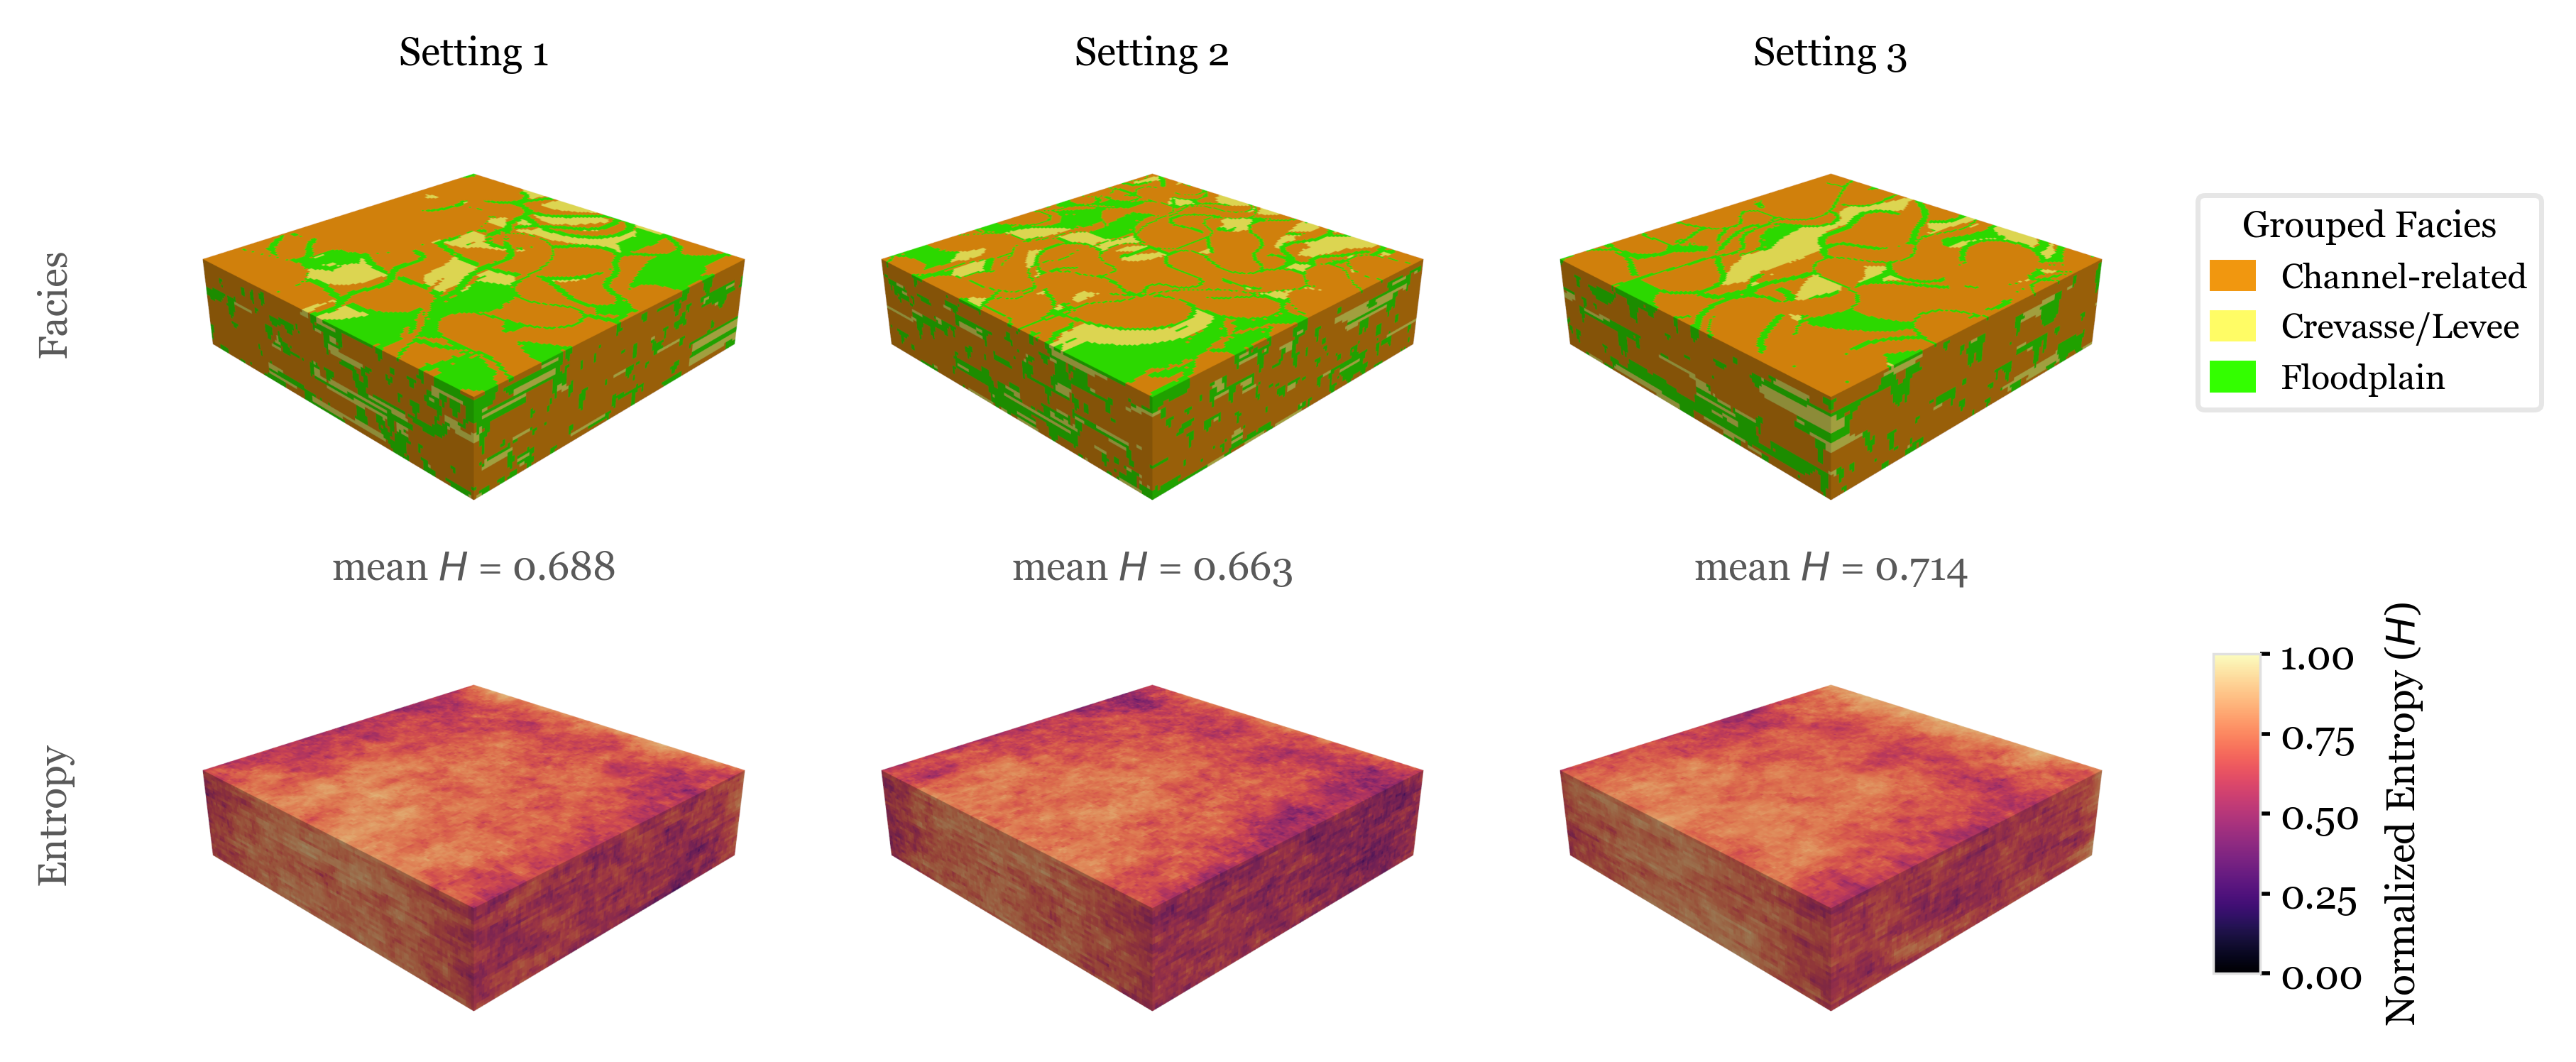
\includegraphics[width=0.99\textwidth]{figures/results/flumy_datasets/all_settings_3d.png}
    \caption{3-dimensional categorical facies realizations (top row) and corresponding voxel-wise normalized spatial entropy ($H$) volumes (bottom row) computed across 1,000~samples for each of the three geological settings. The facies values have been grouped into three classes as defined in Table~\ref{tab:3_facies_grouping}}
    \label{fig:datasets_3d_comparison}
\end{figure} 

From a visual perspective, the 3D facies realizations show no clear differences between the three settings. However, from a multi-dimensional perspective, there is a clear divergence in their structural topology and spatial predictability. This visual similarity occurs because the net-to-gross ratio is fixed at 67\%~across all three settings~(Table~\ref{tab:NEXUS_input}), meaning the total volume of sand is nearly identical. Because of this, looking at single 3D realizations does not reveal the underlying parameter changes~(Figure~\ref{fig:datasets_3d_comparison}, top row). For a more detailed cross-sectional overview of each setting, 2D orthogonal slices~($XY$, $XZ$, and $YZ$) are provided in Appendix~\ref{Appendix:Flumy_datasets}~(Figure~\ref{fig:appendix_flumy_facies_slices}).

This visual ambiguity is resolved when looking at the 2D~\gls{mds} plot~(Figure~\ref{fig:datasets_2d_mds_comparison}), where samples from each setting form clear, separate groups. In this plot, Setting~2 forms a compact cluster in the central area, while Setting~3 shows a much wider spread across the domain. This wider spread in Setting~3 is caused by its larger channel depth~(7~m) and sand-body extension~(120$\times$), which allow for a wider variety of channel geometries. Furthermore, these structural differences are quantitatively supported by the 3D voxel-wise normalized spatial entropy~($H$) volumes~(Figure~\ref{fig:datasets_3d_comparison}, bottom row; see Figure~\ref{fig:appendix_flumy_entropy_slices} for 2D entropy slices). Setting~2 exhibits the lowest mean voxel-wise entropy~($\bar{H} = 0.663$), reflecting a more rigidly constrained channel layout, while Setting~1 shows intermediate variability~($\bar{H} = 0.688$), and Setting~3 displays the highest spatial diversity~($\bar{H} = 0.714$). Additionally, the 3D entropy blocks show lower values near the grid edges due to boundary rules in the FLUMY simulator, as further discussed in Section~\ref{Sec:Post_training_res}. This boundary reduction in entropy is an inherent limitation of FLUMY, as an ideal training dataset should maintain constant spatial entropy throughout the complete volume. Together, these entropy values set a baseline for spatial uncertainty to evaluate the generative diversity of the trained~\gls{gan} models.

\begin{figure}[htbp!]
    \centering
    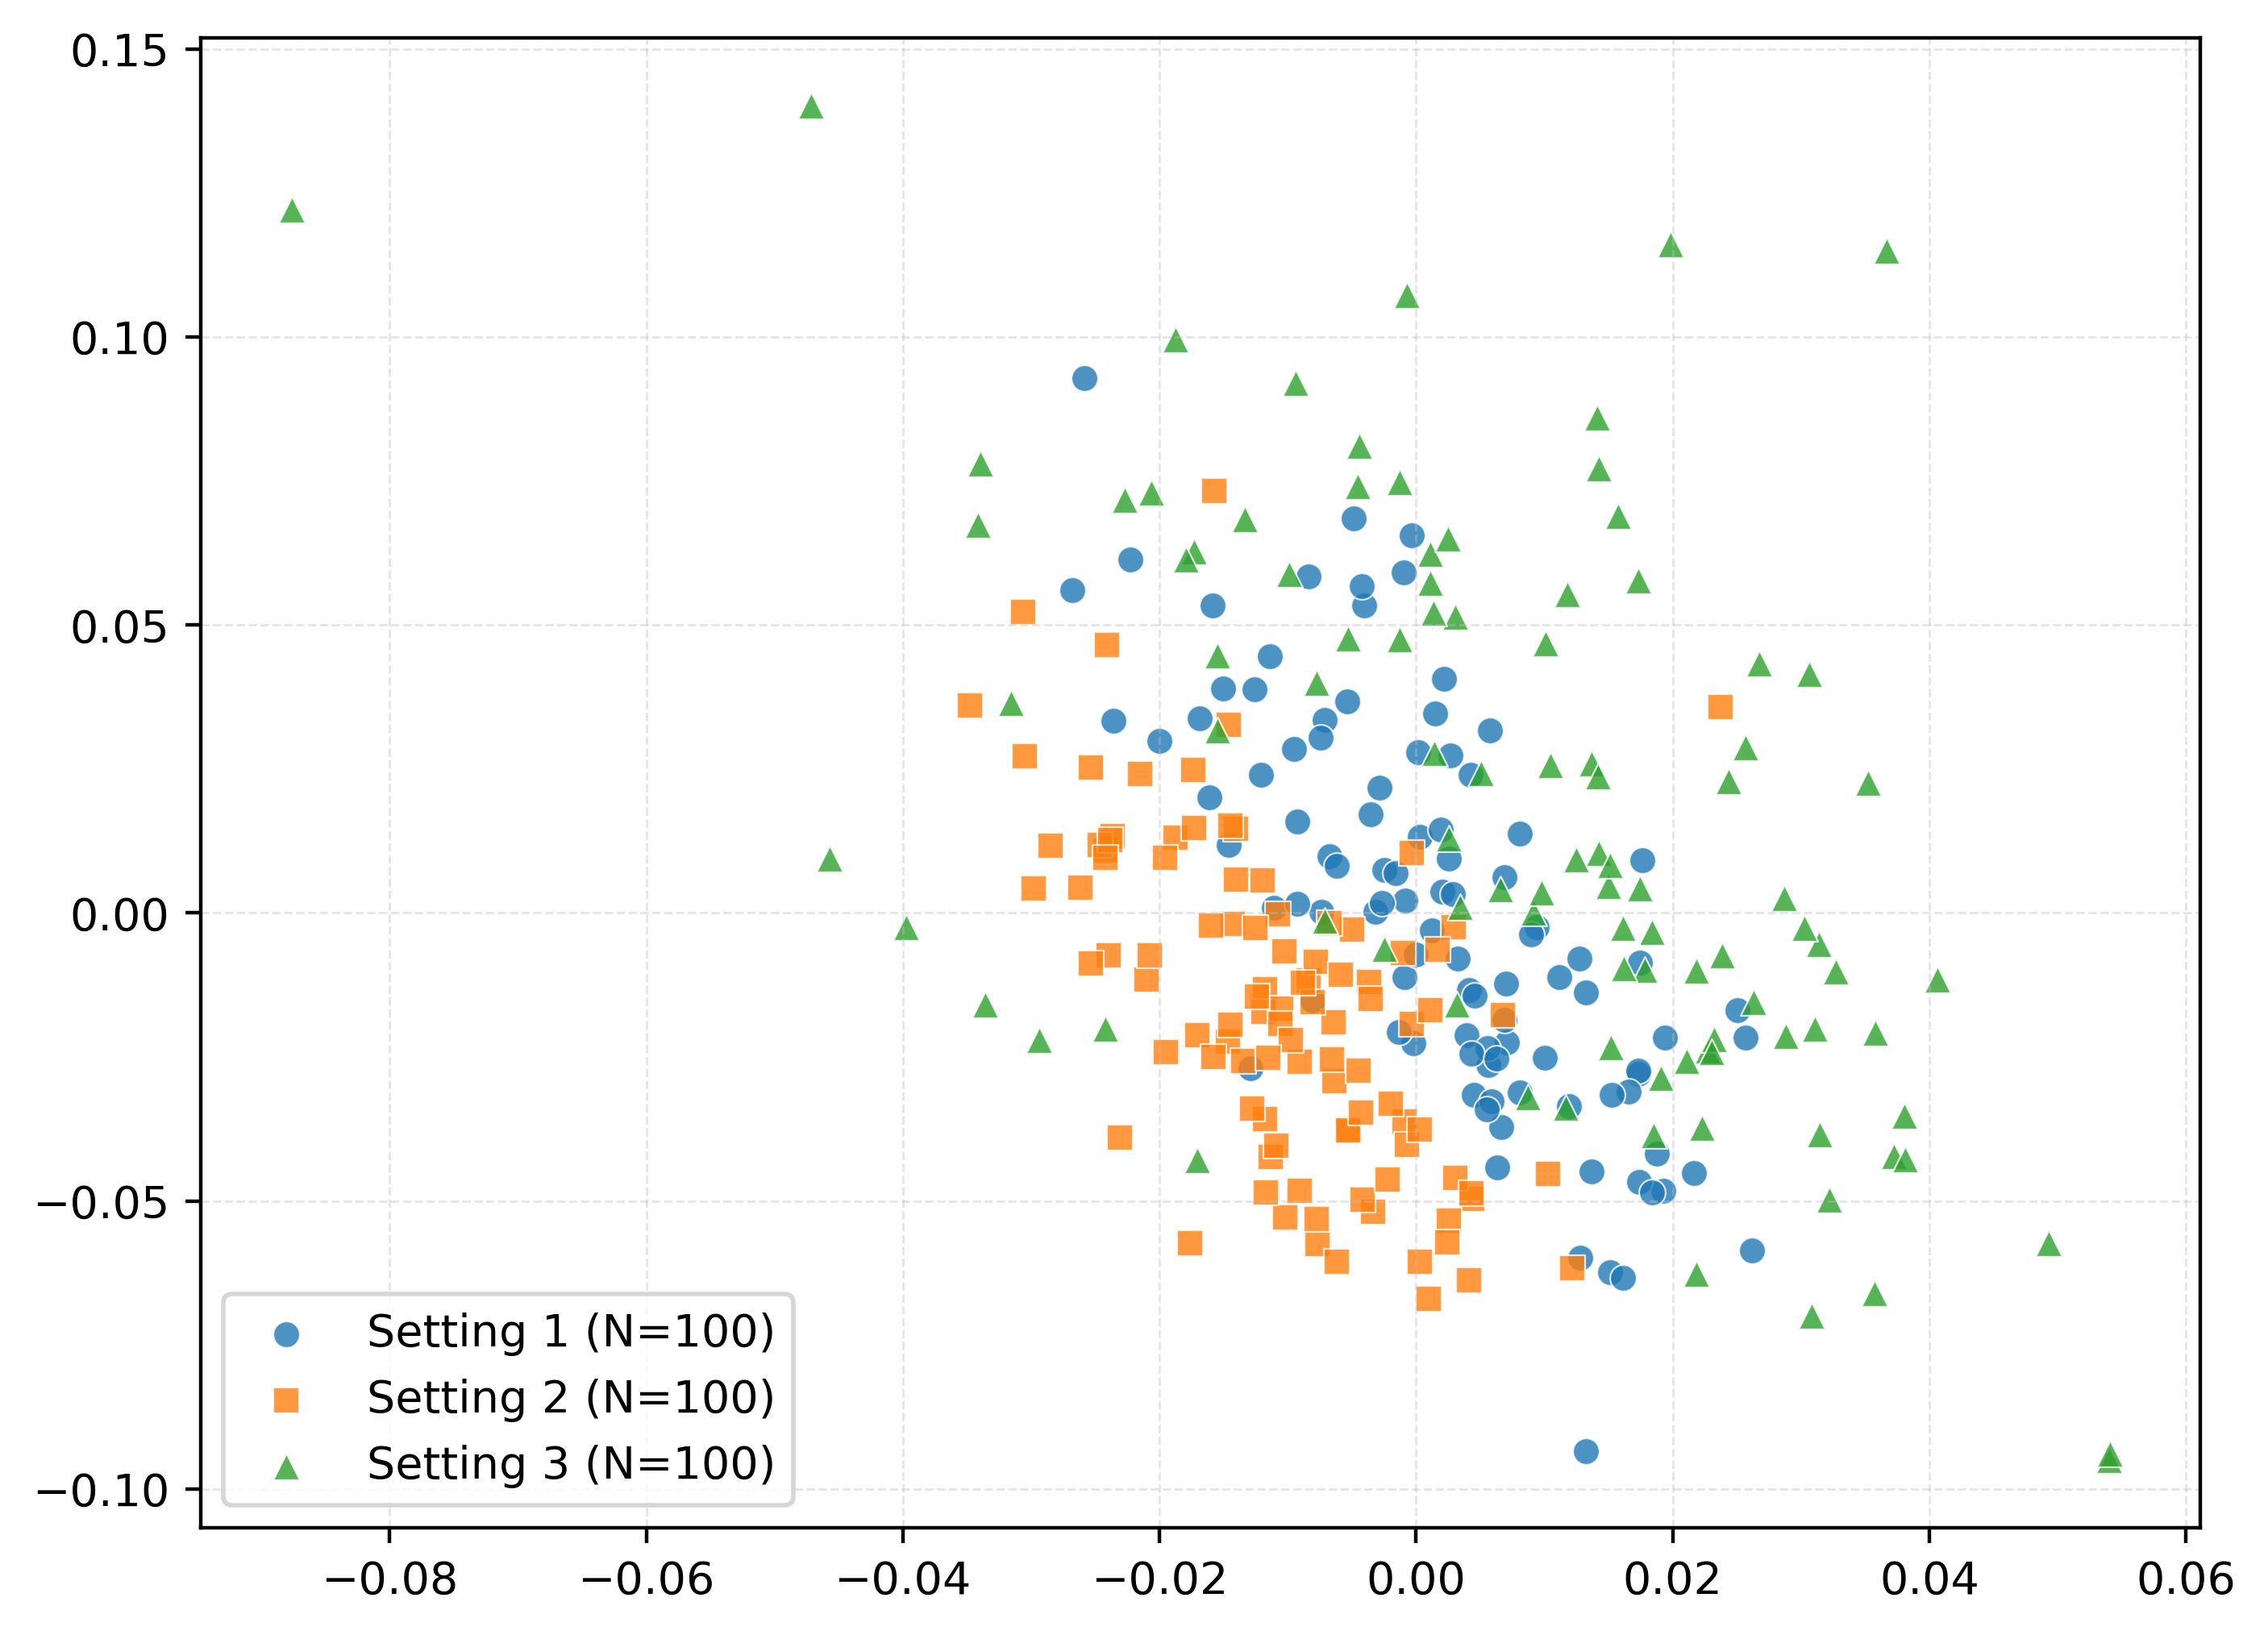
\includegraphics[width=0.95\textwidth]{figures/results/flumy_datasets/2d_mds_all_settings.png}
    \caption{\glsentryshort{mds} projection of 100~random realizations per setting, illustrating structural clustering.}
    \label{fig:datasets_2d_mds_comparison}
\end{figure}   

The volumetric facies composition for each setting is summarized in Table~\ref{tab:comparison_facies_distribution_flumy_samples}.

\begin{table}[htbp!]
    \centering
    \renewcommand{\arraystretch}{1.4}
    \small
    \begin{tabularx}{\textwidth}{Xccc}
        \hline
        \textbf{Facies} & \textbf{Setting 1 (\%)} & \textbf{Setting 2 (\%)} & \textbf{Setting 3 (\%)}\\
        \hline
        \textbf{1: Channel Lag} & 1.6 & 1.8 & 1.8 \\
        \textbf{2: Point Bar} & 67.5 & 66.3 & 65.4 \\
        \textbf{3: Sand Plug} & 1.8 & 1.6 & 1.4 \\
        \textbf{4: Crevasse Splay Core} & 0.0 & 0.0 & 0.0 \\
        \textbf{5: Crevasse Channel} & 0.1  & 0.1 & 0.1 \\
        \textbf{6: Crevasse Splay Delta} & 0.0 & 0.0 & 0.0 \\
        \textbf{7: Levee} & 5.1 & 6.5 & 7.7 \\
        \textbf{8: Overbank} & 10.2 & 11.4 & 11.9 \\
        \textbf{9: Mud Plug} & 13.6 & 12.4 & 11.5 \\
        \hline
    \end{tabularx}
    \caption{Global categorical facies distribution profiles compared across the three synthetic training datasets for all available classes.}
    \label{tab:comparison_facies_distribution_flumy_samples}
\end{table}

Moving from Setting~1 to Setting~3, Table~\ref{tab:comparison_facies_distribution_flumy_samples} shows a gradual increase in Levee~(5.1\%~to 7.7\%) and Overbank facies~(10.2\%~to 11.9\%), along with a slight decrease in Mud Plugs~(13.6\%~to 11.5\%). This trend reflects more overbank flooding caused by deeper channels and wider sand bodies. However, Table~\ref{tab:comparison_facies_distribution_flumy_samples} also reveals a severe class imbalance across the datasets. The dominant point bar facies occupies over 65\%~of the total volume, while several minority categories are heavily suppressed. In particular, Facies~4, 5, and~6 each make up only 0.0\%~to 0.1\%~of the volume, which is a known limitation of the default FLUMY NEXUS parameters. This strong imbalance creates an optimization challenge during adversarial training. Because standard~\gls{gan} loss functions treat every voxel with equal weight, the discriminator focuses mostly on evaluating the dominant facies. As a result, the generator learns large-scale channel structures well but struggles to capture the nuances of rare minority facies. This discrepancy must be taken into account during subsequent model evaluations, particularly for localized well-conditioning metrics.

When transitioning from the detailed 9-class categorization to the upscaled 3-class configuration, the secondary class naturally expands to constitute approximately 5\%~to 8\%~of the total volume. By design, these grouped facies proportions closely match the empirical proportions interpreted from the real cored and logged intervals of the DEL-GT-01 and DEL-GT-02-S2 wells~(see Figure~\ref{fig:well_data}). Therefore, while the original 9-class prior suffers from severe generative constraints under default settings, this upscaled interpretation successfully aligns the dataset's global facies distributions with the target reservoir characteristics.

\section{Post Training Generative Results}\label{Sec:Post_training_res}
All models and experimental runs described in the following subsections were trained on two NVIDIA-A100 GPUs with 80~GB of unified memory each. When trained for 25~epochs on 20,000~samples, the training time ranged between 3~and 5~hours depending on the hyperparameter setup, whereas models trained for 100~epochs required approximately 20~hours.

\subsection{Hyperparameter Tuning}\label{Sec:Hyperparam_results}
An ablation study was conducted to determine the optimal GAN architecture and regularization configuration for 3D fluvial geomodelling. Eight model configurations were evaluated by monitoring training \gls{swd} loss curves alongside test \gls{jsd}, \gls{msswd}, and 3D spatial entropy metrics~(Table~\ref{tab:ablation_study} and Figure~\ref{fig:ablation_study}). Each model reserved 10\%~of its training data exclusively for validation, with final evaluations computed on an ensemble of 1,000~generated realizations against a 1,000-sample test set. This setup isolates the individual effects of network depth, discriminator regularization frequency, dataset volume, and update intervals.

\begin{table}[htbp!]
    \centering
    \renewcommand{\arraystretch}{1.4}
    \resizebox{\textwidth}{!}{%
    \begin{tabular}{cccccccc}
        \hline
        \textbf{Model} & \textbf{Epochs}& \textbf{disc penalty} & \textbf{double conv} & \textbf{double resblock} & \textbf{\gls{jsd} $\downarrow$} & \textbf{\gls{msswd} $\downarrow$} & \textbf{mean $H_{norm}$ $\uparrow$}\\
        \hline
        1 & 25 & no & off & off & 0.0718 $\pm$ 0.0157 & 0.08865 & 0.515 \\
        2 & 25 & no & on & off & 0.1161 $\pm$ 0.0243 & 0.06842 & 0.430 \\
        3 & 25 & no & on & on & 0.0458 $\pm$ 0.0076 & 0.08271 & 0.637 \\
        4 & 25 & 32 & on & on & 0.0612 $\pm$ 0.0314 & 0.09224 & 0.629 \\
        \textbf{5} & \textbf{25} & \textbf{16} & \textbf{on} & \textbf{on} & \textbf{0.0155 $\pm$ 0.0067} & \textbf{0.07986} & \textbf{0.704} \\
        6 & 25 & 1 & on & on & 0.0202 $\pm$ 0.0038 & 0.07690 & 0.614 \\
        7 & 25 & 16 & on & on & 0.1190 $\pm$ 0.0324 & 0.11924 & 0.393 \\
        8 & 25 & 16 & on & on & 0.0278 $\pm$ 0.0045 &  0.13389 & 0.623 \\
        \hline
    \end{tabular}%
    }
    \caption{Overview of hyperparameters and evaluation metrics of each model. Model~5, based on Architecture~4 by~\parencite{rongier2025atowards}, yields the best \glsentryshort{jsd} and second-best \glsentryshort{msswd} value.}
    \label{tab:ablation_study}
\end{table}

\begin{figure}[htbp]
    \centering
    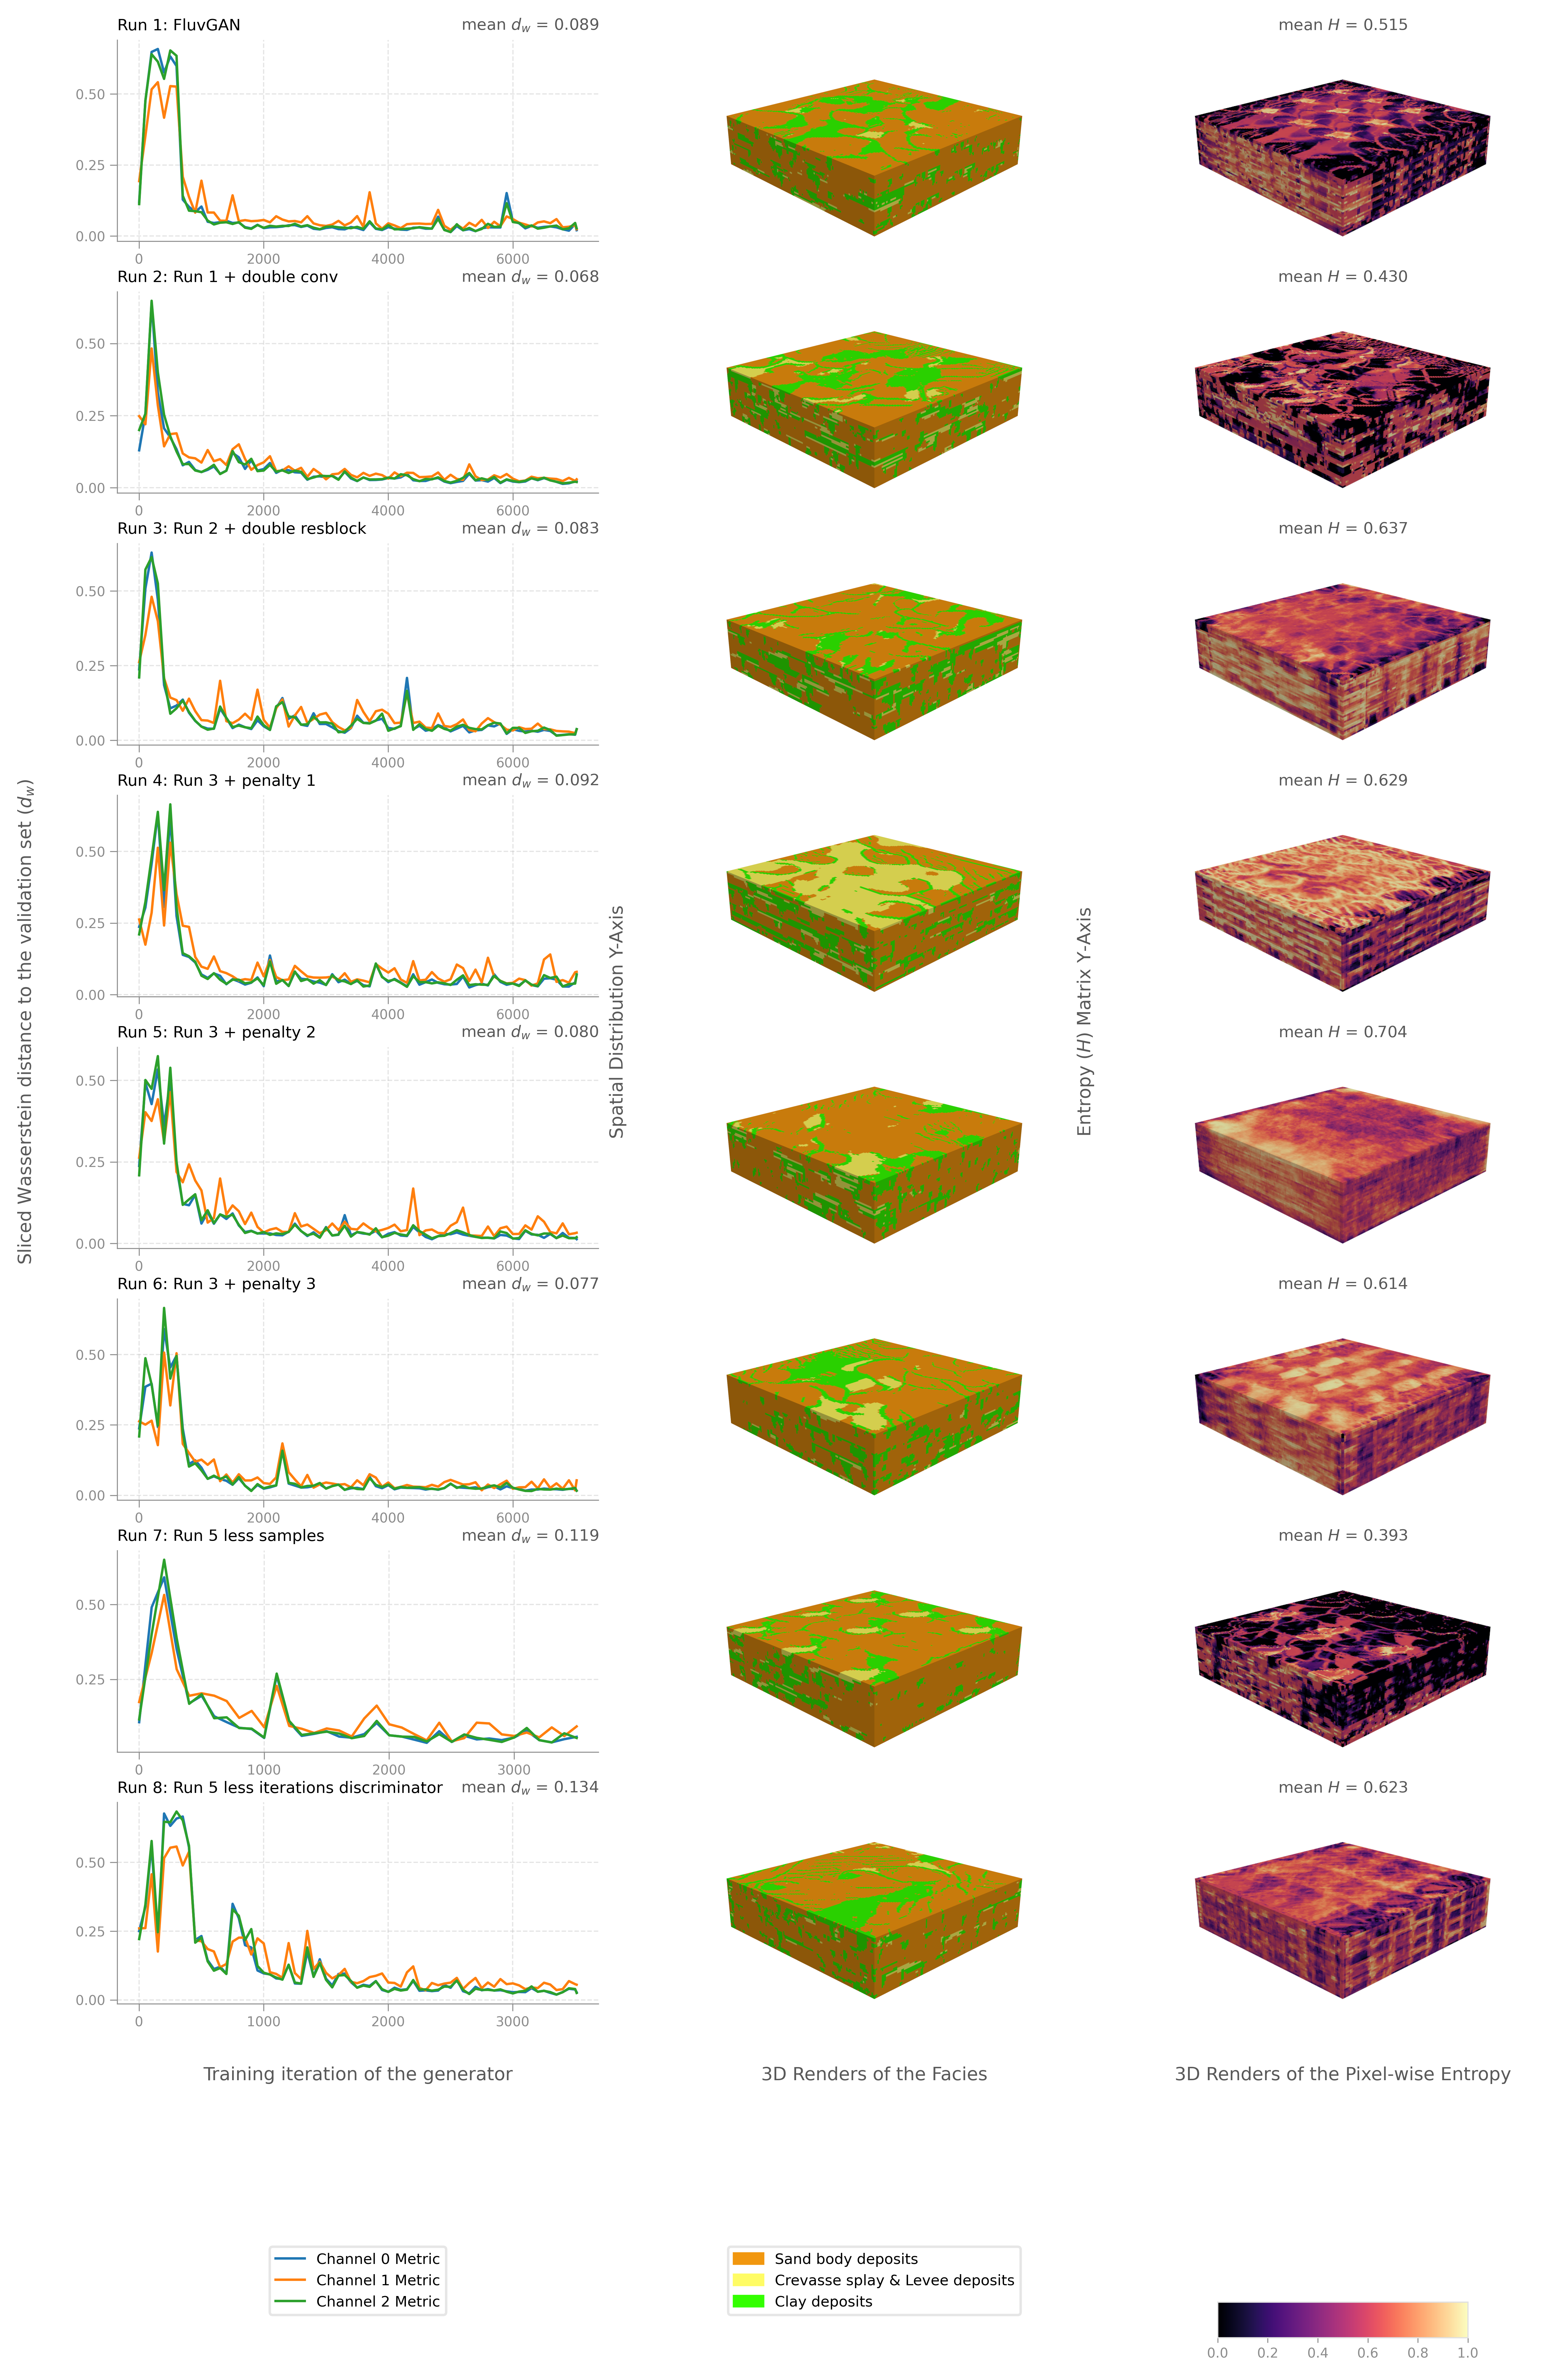
\includegraphics[width=0.95\textwidth]{figures/results/hyperparameter_tuning/Ablation_study.png}
    \caption{Ablation study starting from \glsentryshort{fluvgan} and progressively adding/adjusting parameters to observe their effect on training, geological plausibility, and sample diversity.~\textit{Model 1:} Standard \glsentryshort{fluvgan} architecture from~\parencite{rongier2025atowards}.~\textit{Model 2:} Addition of double convolutional layers.~\textit{Model 3:} Addition of double residual blocks on top of double convolutions.~\textit{Model 4:} Addition of a discriminator penalty every 32~iterations.~\textit{Model 5:} Discriminator penalty applied every 16~iterations.~\textit{Model 6:} Discriminator penalty applied every iteration.~\textit{Model 7:} Model~5 hyperparameters with reduced dataset of 10,000~training samples.~\textit{Model 8:} Model~5 hyperparameters with discriminator updated every 2~iterations.}
    \label{fig:ablation_study}
\end{figure}

Model~5 achieves the most balanced performance between statistical accuracy and spatial diversity among the tested configurations. It produces the lowest \gls{jsd}~($0.0155 \pm 0.0067$) and the second-lowest \gls{msswd}~($0.07986$), indicating strong multi-scale distribution matching~(Table~\ref{tab:ablation_study}). Furthermore, it generates the highest normalized voxel-wise entropy ($\bar{H}_{norm} = 0.704$), which closely matches the Setting~2 baseline ($\bar{H}_{norm} = 0.692$) and avoids the severe mode collapse seen in simpler architectures. Across all stable runs, the \gls{swd} loss curves show an initial error spike during the first $\sim 500$~iterations before stabilizing after approximately 2,000~iterations, indicating rapid multi-scale convergence early in the training cycle.

Network depth, discriminator regularization frequency, and training dataset volume significantly influence GAN training stability. The base \gls{fluvgan} architecture (Model~1) suffers from noticeable mode collapse ($\bar{H}_{norm} = 0.515$), and adding double convolutions alone without residual blocks (Model~2) further degrades \gls{jsd}~($0.1161$) and reduces entropy ($\bar{H}_{norm} = 0.430$). Stable training is achieved only after introducing both double convolutions and residual blocks (Model~3, $\bar{H}_{norm} = 0.637$), while applying an R1 gradient penalty every 16~iterations (Model~5) provides the most balanced training dynamics. In contrast, applying the penalty at every iteration (Model~6) produces a distinct checkerboard artifact in the 3D entropy volume (Figure~\ref{fig:ablation_study}). Furthermore, halving the training dataset to 10,000~samples (Model~7) triggers substantial mode collapse ($\text{JSD} = 0.1190, \bar{H}_{norm} = 0.393$), while updating the discriminator every second iteration (Model~8) deteriorates multi-scale structural matching ($\text{MSSWD} = 0.13389$).

\subsection{Unconstrained Model Results}
Extending training from 25~epochs to 100~epochs (Model~5.1) reproduces realistic fluvial geometries, but retains characteristic GAN structural artifacts. Both Models~5 and~5.1 reproduce realistic sinuous point bars with central mudplugs, adjacent floodplains, and levee deposits (Figure~\ref{fig:2D_Z_slices_models_5(1)_and_flumy}). However, visual inspection of 2D horizontal slices also reveals closed-loop channel artifacts~\circled{1}, previously documented by~\textcite{sun2023geological}, along with isolated single-voxel noise~\circled{2}. Because 2D visual inspection cannot evaluate full 3D spatial continuity, quantitative volumetric metrics are necessary to properly assess model quality.

\begin{table}[htbp!]
    \centering
    \renewcommand{\arraystretch}{1.4}
    \small
    \begin{tabularx}{\textwidth}{Xcccccc}
        \hline
        \textbf{Name}& \textbf{Epochs} & \textbf{\gls{jsd} $\downarrow$} & \textbf{\gls{msswd} $\downarrow$} & \textbf{Mean $H_{norm}\uparrow$} & \textbf{$n$ Unique Patterns} & \\
        \hline
        Setting 2 & -   & -               & -            & 0.692          & 2,949,220 \\
        Model 5   & 25  & 0.0146          & 0.080        & 0.704          & 3,846,513 \\
        Model 5.1 & 100 & \textbf{0.0132} & \textbf{0.078} & \textbf{0.684} & \textbf{3,727,836} \\
        \hline
    \end{tabularx}
    \caption{Overview of hyperparameters and evaluation metrics of each model ($N = 100$~realizations). Model~5, based on Architecture~4 by~\parencite{rongier2025atowards}, yields the best \glsentryshort{jsd} and second-best \glsentryshort{msswd} value.}
    \label{tab:model_5_epoch_comparison}
\end{table}

\begin{figure}[htbp!]
    \centering
    \begin{tikzpicture}
        \node[anchor=south west, inner sep=0] (image) at (0,0) {%
            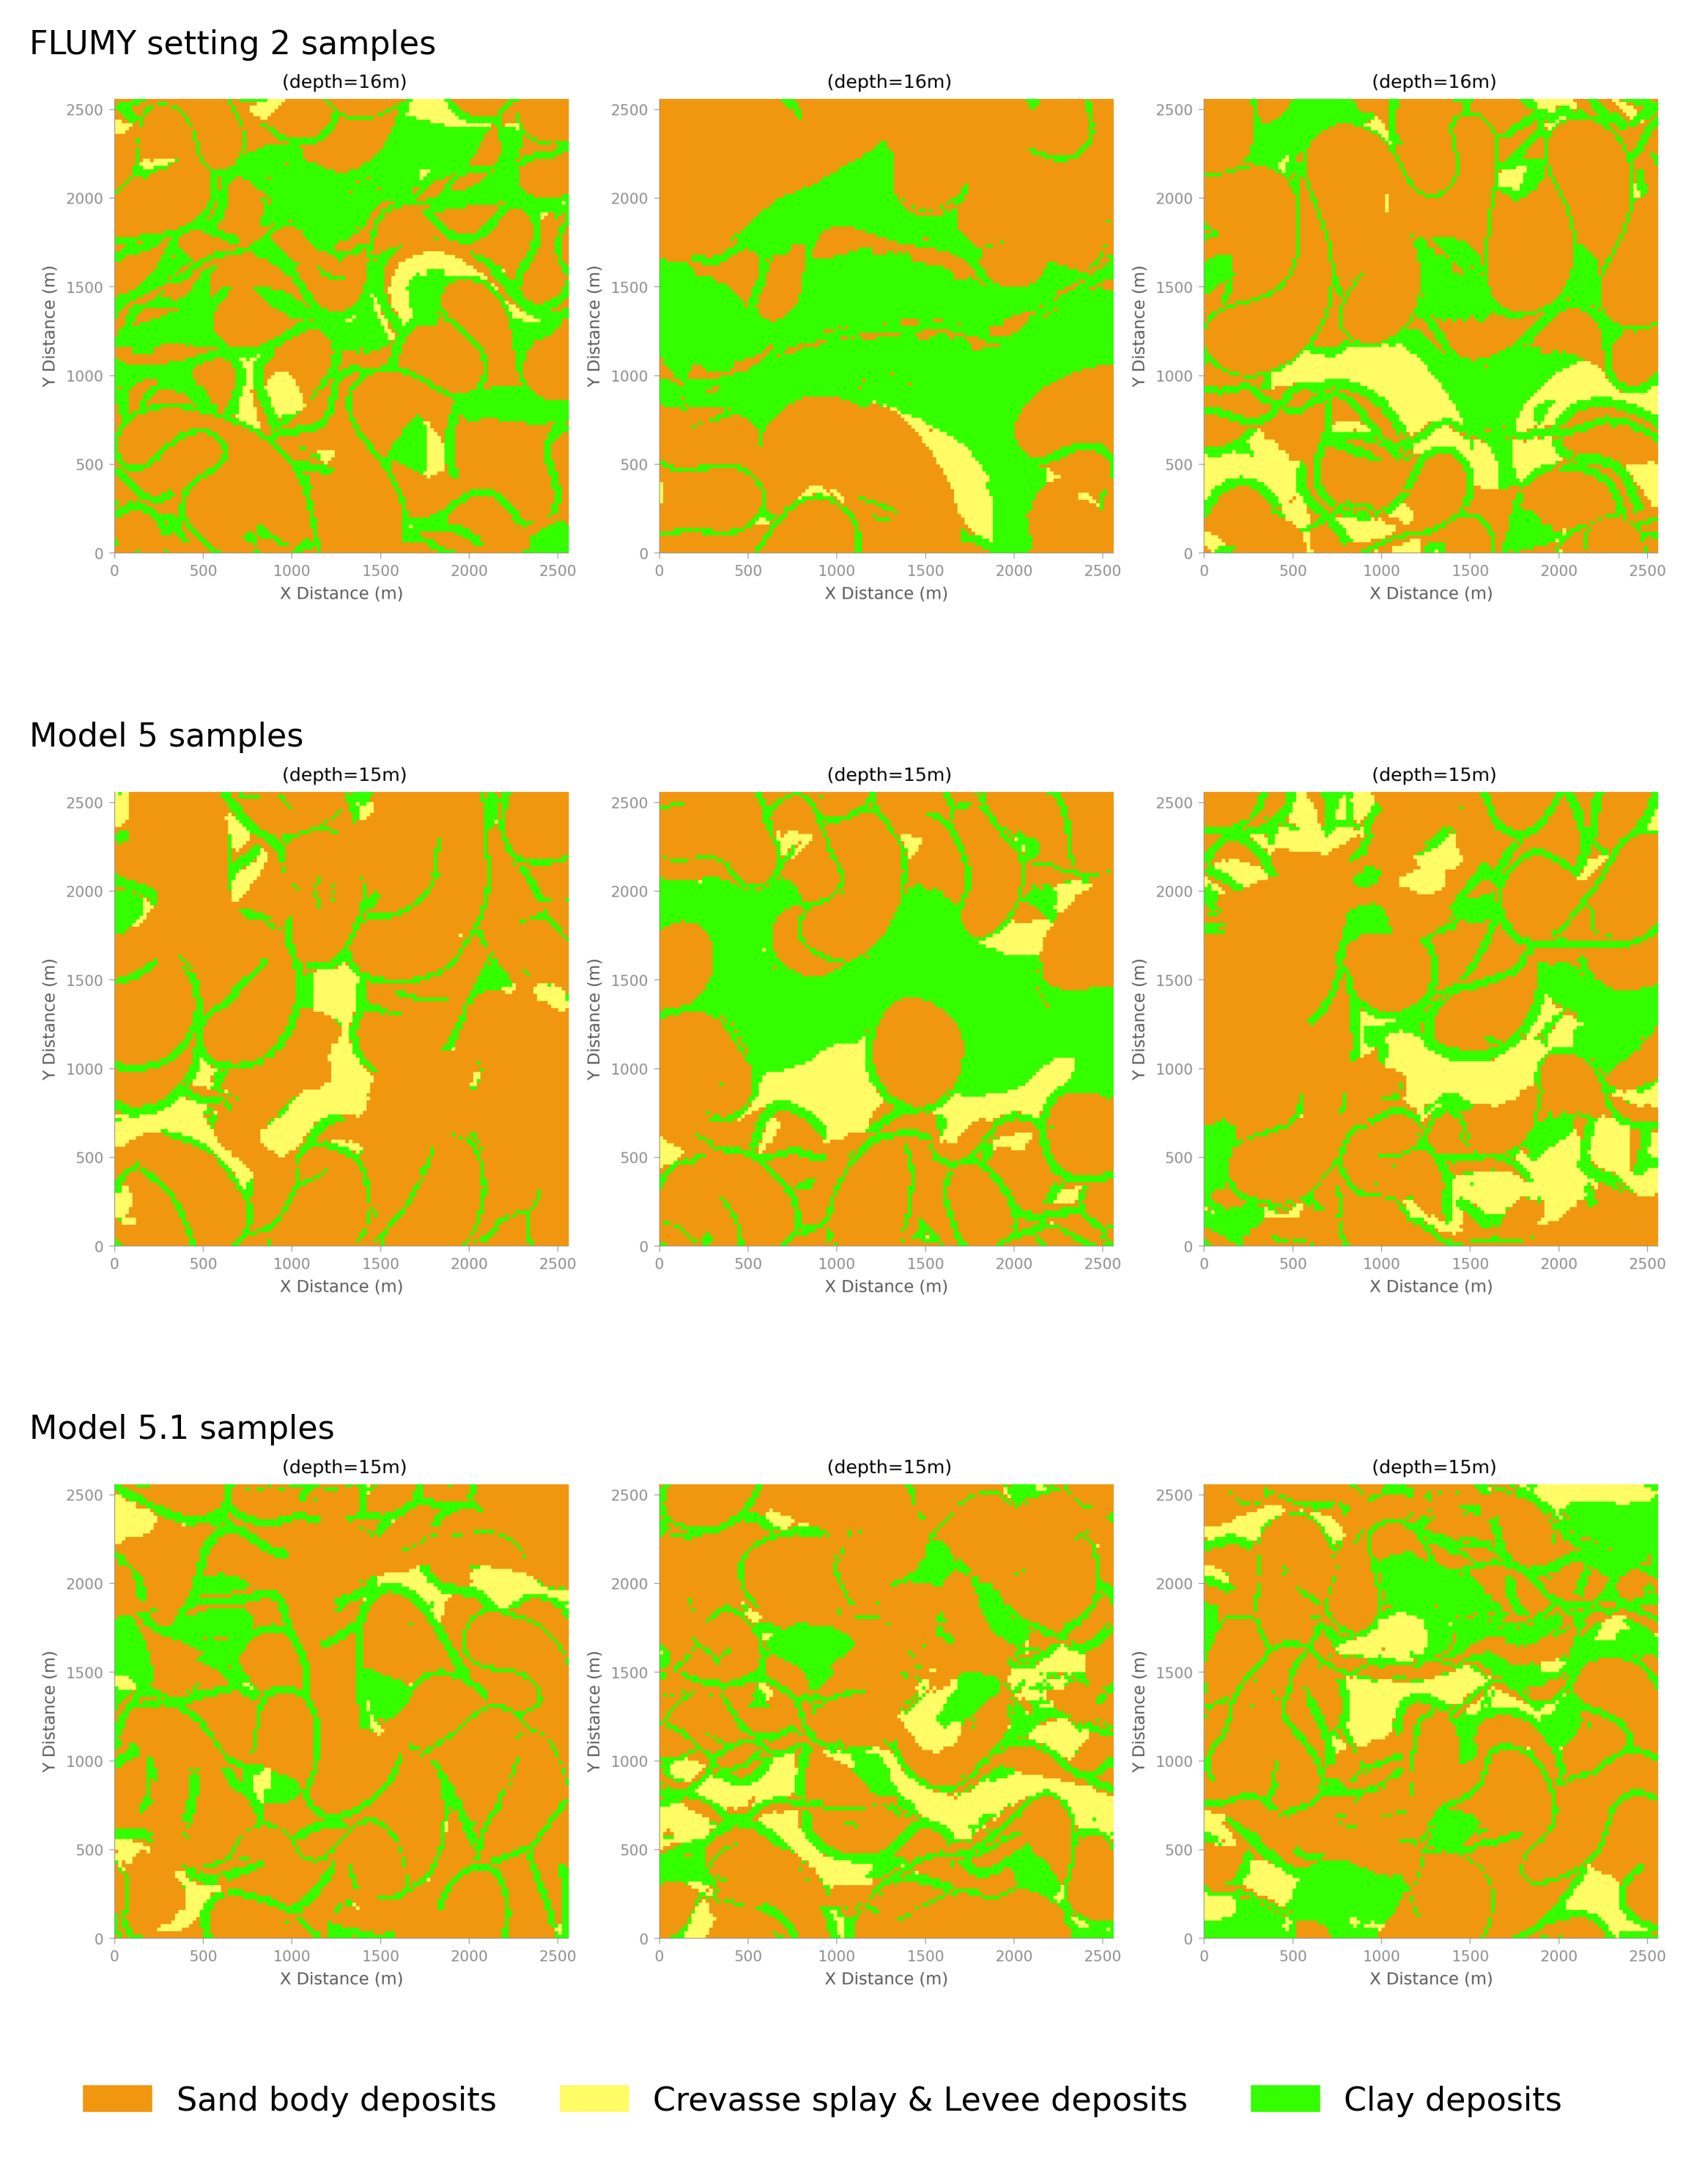
\includegraphics[width=0.99\linewidth]{figures/results/cgan_unconstrained_performance/master_combined_grid_3x1.png}%
        };
        \begin{scope}[x={(image.south east)}, y={(image.north west)}]
            \node[draw=black, fill=white, circle, inner sep=1.5pt, font=\small\bfseries, line width=1pt] 
                at (0.55, 0.52) {1};
            \node[draw=black, fill=white, circle, inner sep=1.5pt, font=\small\bfseries, line width=1pt] 
                at (0.8, 0.56) {1};
            \node[draw=black, fill=white, circle, inner sep=1.5pt, font=\small\bfseries, line width=1pt] 
                at (0.56, 0.24) {2};
        \end{scope}
    \end{tikzpicture}
    \caption{2D slices taken from the Z-axis at depth 16~m of samples from 1) the \textit{FLUMY} test dataset, 2) Model~5 (trained for 25~epochs), and 3) Model~5.1 (trained for 100~epochs). \circled{1}~denotes areas of closed loop structures, whereas \circled{2}~denotes areas with single isolated voxels.}
    \label{fig:2D_Z_slices_models_5(1)_and_flumy}
\end{figure}

Extended training to 100~epochs yields diminishing returns, offering only marginal statistical differences compared to the 25-epoch baseline. The global \gls{jsd} metric improves slightly from 0.0146 to 0.0132, while mean voxel-wise entropy shows a minor reduction from 0.704 to 0.684~(Table~\ref{tab:model_5_epoch_comparison}). Both models exhibit an approximate 30\%~inflation in unique local patterns compared to the reference dataset ($3.8\text{M}$ and $3.7\text{M}$ vs.~$2.9\text{M}$). While multidimensional scaling projections of \gls{msswd}~(Figure~\ref{fig:2d_mds_unconstrained_models_5_and_5_1}) visually suggest that Model~5.1 might have a slightly better overlap with the test dataset cluster of setting 2 compared to Model~5, this subtle difference is difficult to confirm definitively. A formal clustering algorithm would be required to quantitatively verify this observation, which could not be performed within the scope of this study. Consequently, based purely on the \gls{mds} projections applied here, the additional 75~epochs do not appear to substantially alter the underlying generative manifold.

Connectivity analysis indicates that both models capture primary facies clustering, but exhibit excessive small-scale voxel fragmentation. Both configurations noticeably overestimate the frequency of isolated single-voxel blobs in the Crevasse Splay \& Levee and Clay facies~(Figure~\ref{fig:model_5_connectivity_distributions}), which directly accounts for the 30\%~inflation in unique local patterns. For large channel sand bodies ($> 10^3$~voxels), both models closely follow the reference FLUMY connectivity distribution. Model~5.1 shows a modest improvement in intermediate cluster sizes ($10^1$~to $10^3$~voxels), suggesting that additional training epochs slightly enhance facies continuity despite persistent fine-scale noise.

\begin{figure}[ht!]
    \centering
    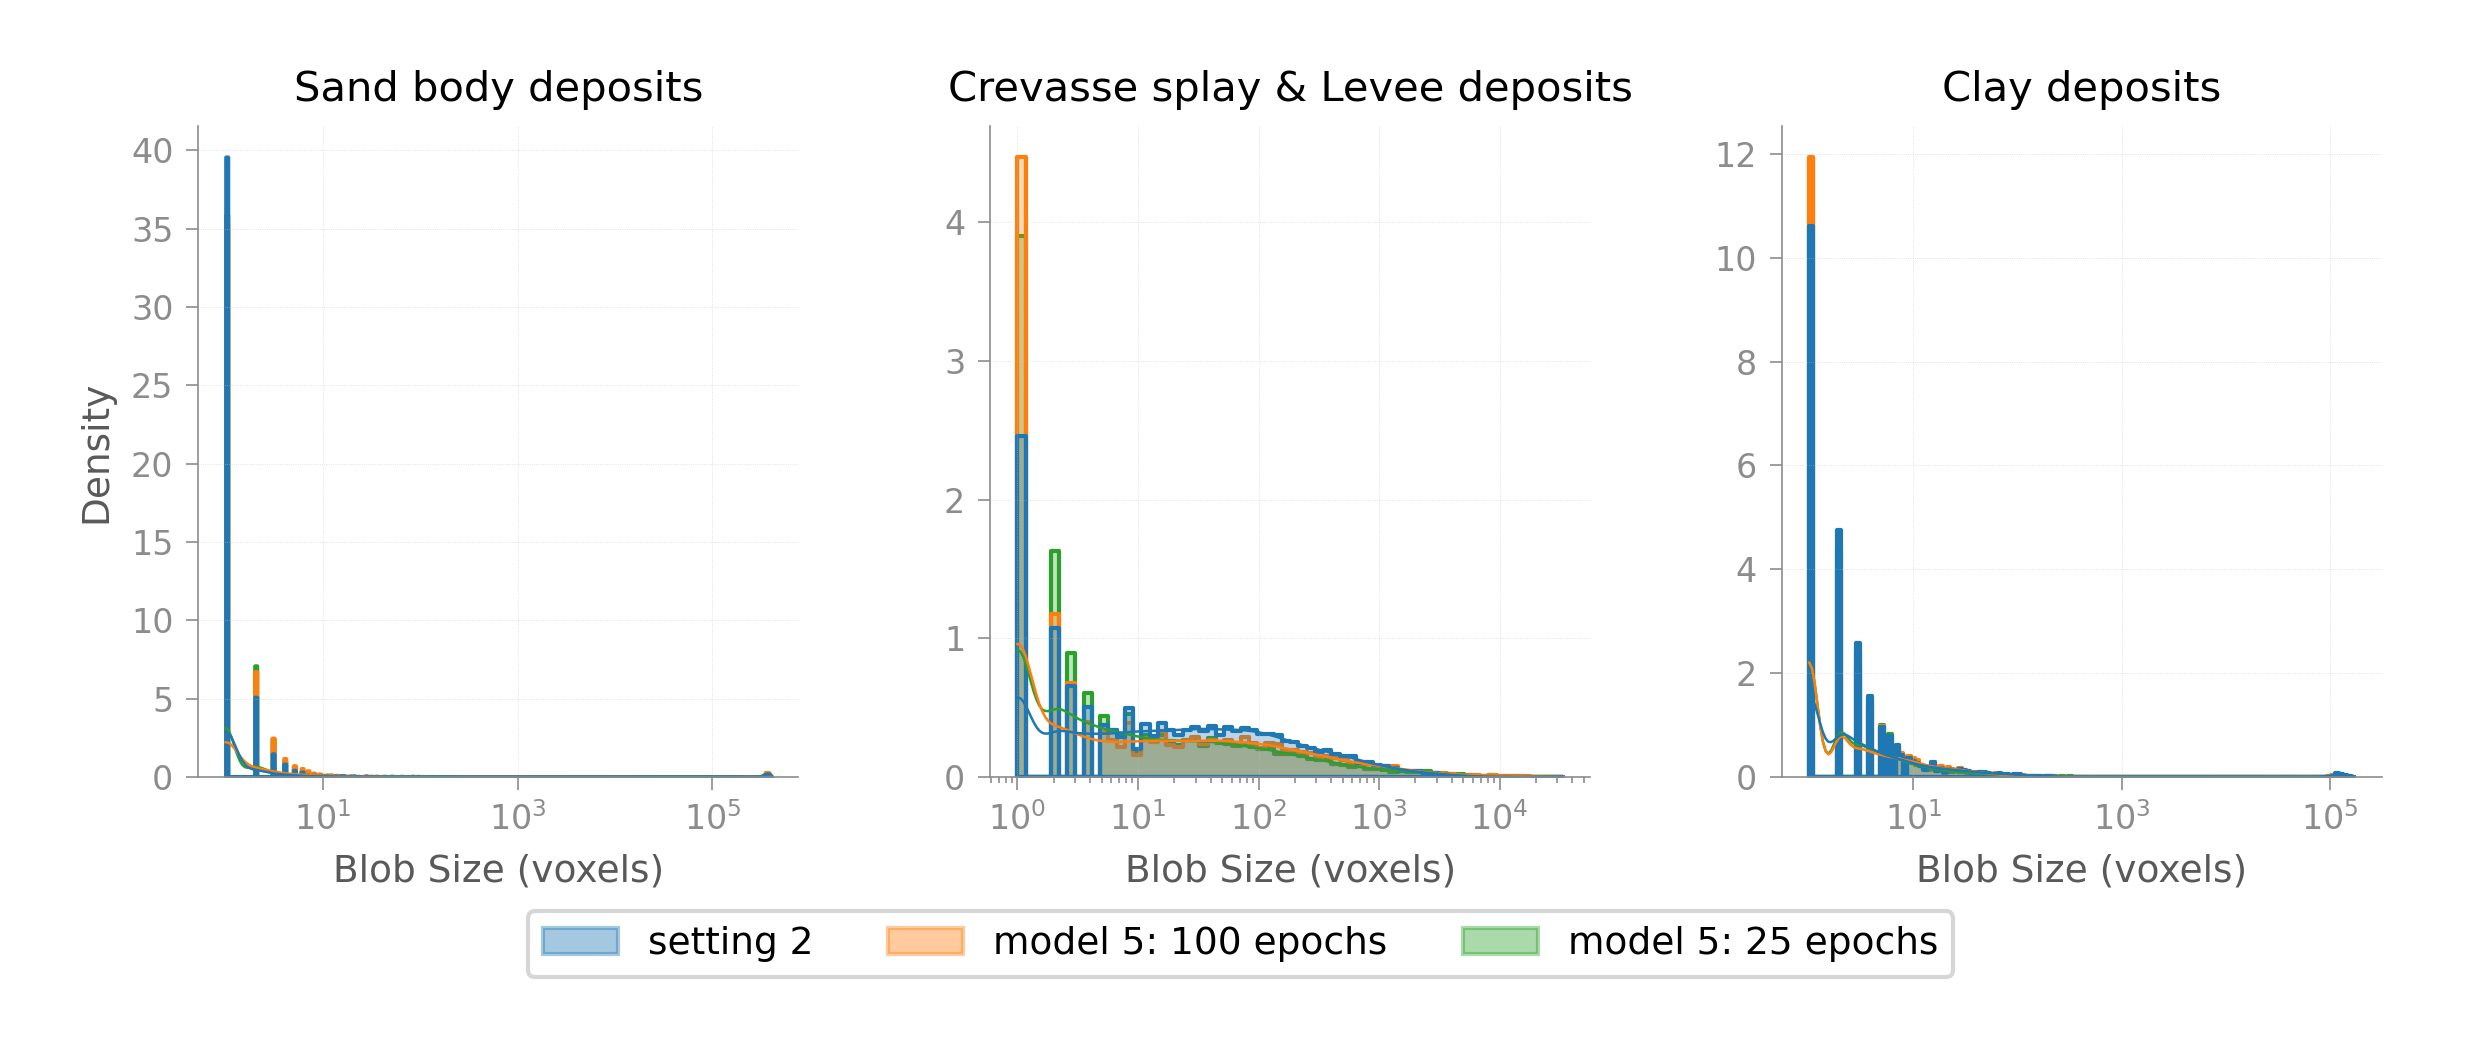
\includegraphics[width=0.9\textwidth]{figures/results/cgan_unconstrained_performance/combined_facies_connectivity_analysis.png}
    \caption{Connectivity analysis plot of the test dataset, illustrating the ability to recreate blob sizes of Model~5 for 25~and 100~training epochs.}
    \label{fig:model_5_connectivity_distributions}
\end{figure}

Vertical entropy and divergence profiles indicate that prolonged training restricts vertical generative variance. In the baseline dataset (Setting~2), normalized entropy remains relatively stable across all 32~vertical slices ($\approx 0.69$, Figure~\ref{fig:H_norm_over_Z_axes}). Model~5 (25~epochs) closely mirrors this vertical baseline consistency, whereas Model~5.1 (100~epochs) displays a marked decline in entropy at the upper and lower boundary slices. Furthermore, \gls{jsd} curves show that generative divergence is primarily concentrated at the vertical boundaries ($Z=0\text{--}3$ and $Z=28\text{--}31$), while remaining low ($\approx 0.01$) across the central reservoir interval.

\begin{figure}[ht!]
    \centering
    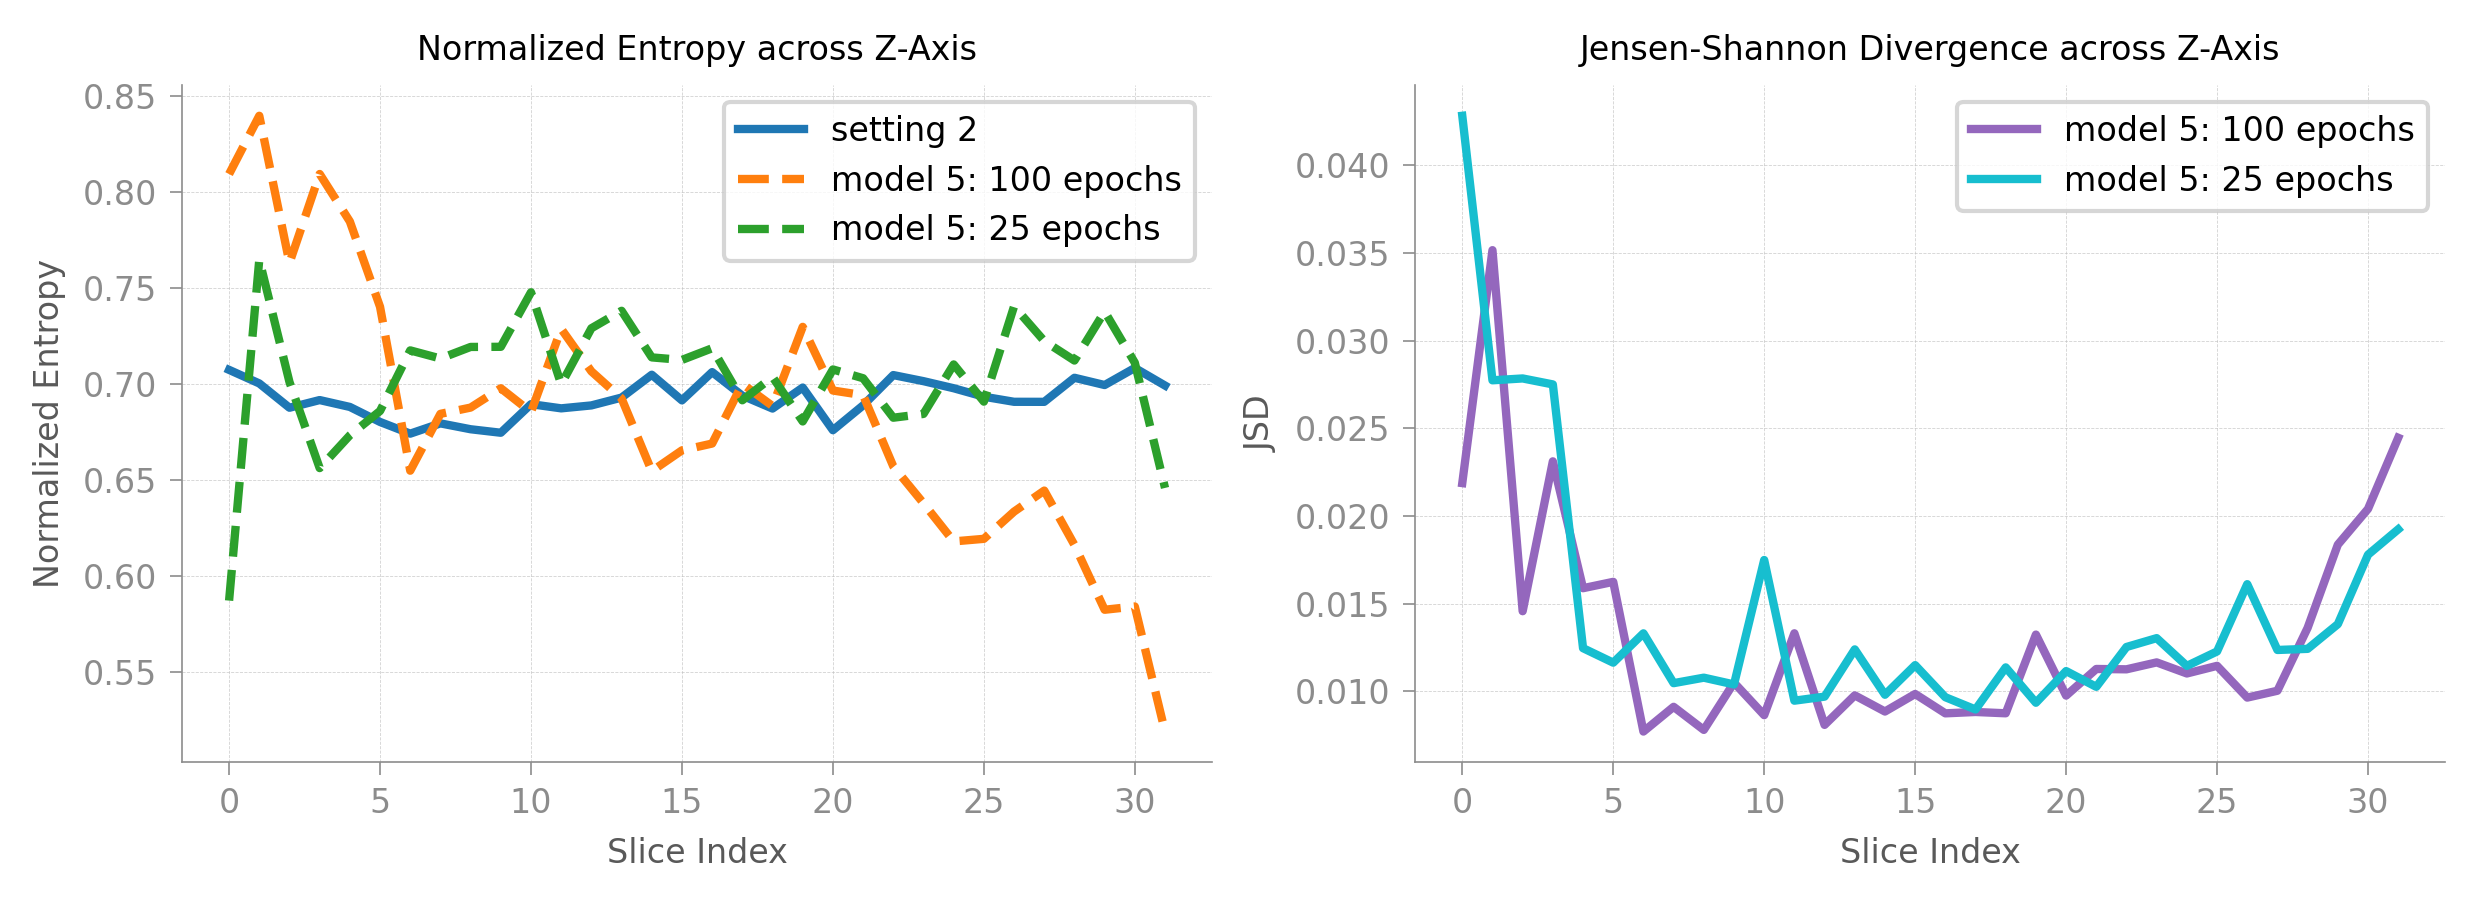
\includegraphics[width=0.9\textwidth]{figures/results/cgan_unconstrained_performance/combined_H_and_JSD_metrics_axis_Z.png}
    \caption{Comparison of the \glsentryshort{jsd} normalized voxel-wise entropy across the Z, Y, and X axes. The decline in Z-axis entropy for Model~5.1 highlights a loss in stochastic diversity.}
    \label{fig:H_norm_over_Z_axes}
\end{figure}

Horizontal entropy profiles reveal spatial non-stationarity and boundary constraints inherited from the process-based FLUMY simulations. Along the Y-axis, an inverted U-shaped entropy curve reflects lateral boundary conditions that confine channel meandering to the central domain ($Y=64$) while suppressing architectural variety near the edges ($Y=0$ and $Y=128$). Along the X-axis, a distinct U-shaped curve with an entropy drop around slices 20~to 30 marks a fixed upstream sediment inlet or nodal avulsion point. This shows that while vertical depositional properties remain stationary across depth, the GAN faithfully reproduces the deterministic boundary constraints present in the training data.

% ----------------------------------------------------
% ------- Additional tested models --------
% ----------------------------------------------------
\subsection{High-Fidelity and Multi-Prior Models}
To evaluate the operational limits of the generative framework, two challenging scenarios were tested: a high-fidelity model and a multi-prior model. The high-fidelity model maintained all nine original facies classes on Setting~2 to evaluate performance under severe class imbalance. In contrast, the multi-prior model used the grouped 3-class configuration, but was trained on a pooled dataset of 30,000~samples spanning Settings~1, 2, and~3 to test whether a single model can capture diverse geological rules. Both configurations were trained for 25~epochs using Model~5 hyperparameters, with results summarized in Table~\ref{tab:high_fidelity_multiprior_comparison} and Figure~\ref{fig:2D_Z_slices_models_hf_all_set_and_flumy}.

\begin{figure}[htbp!]
    \centering
    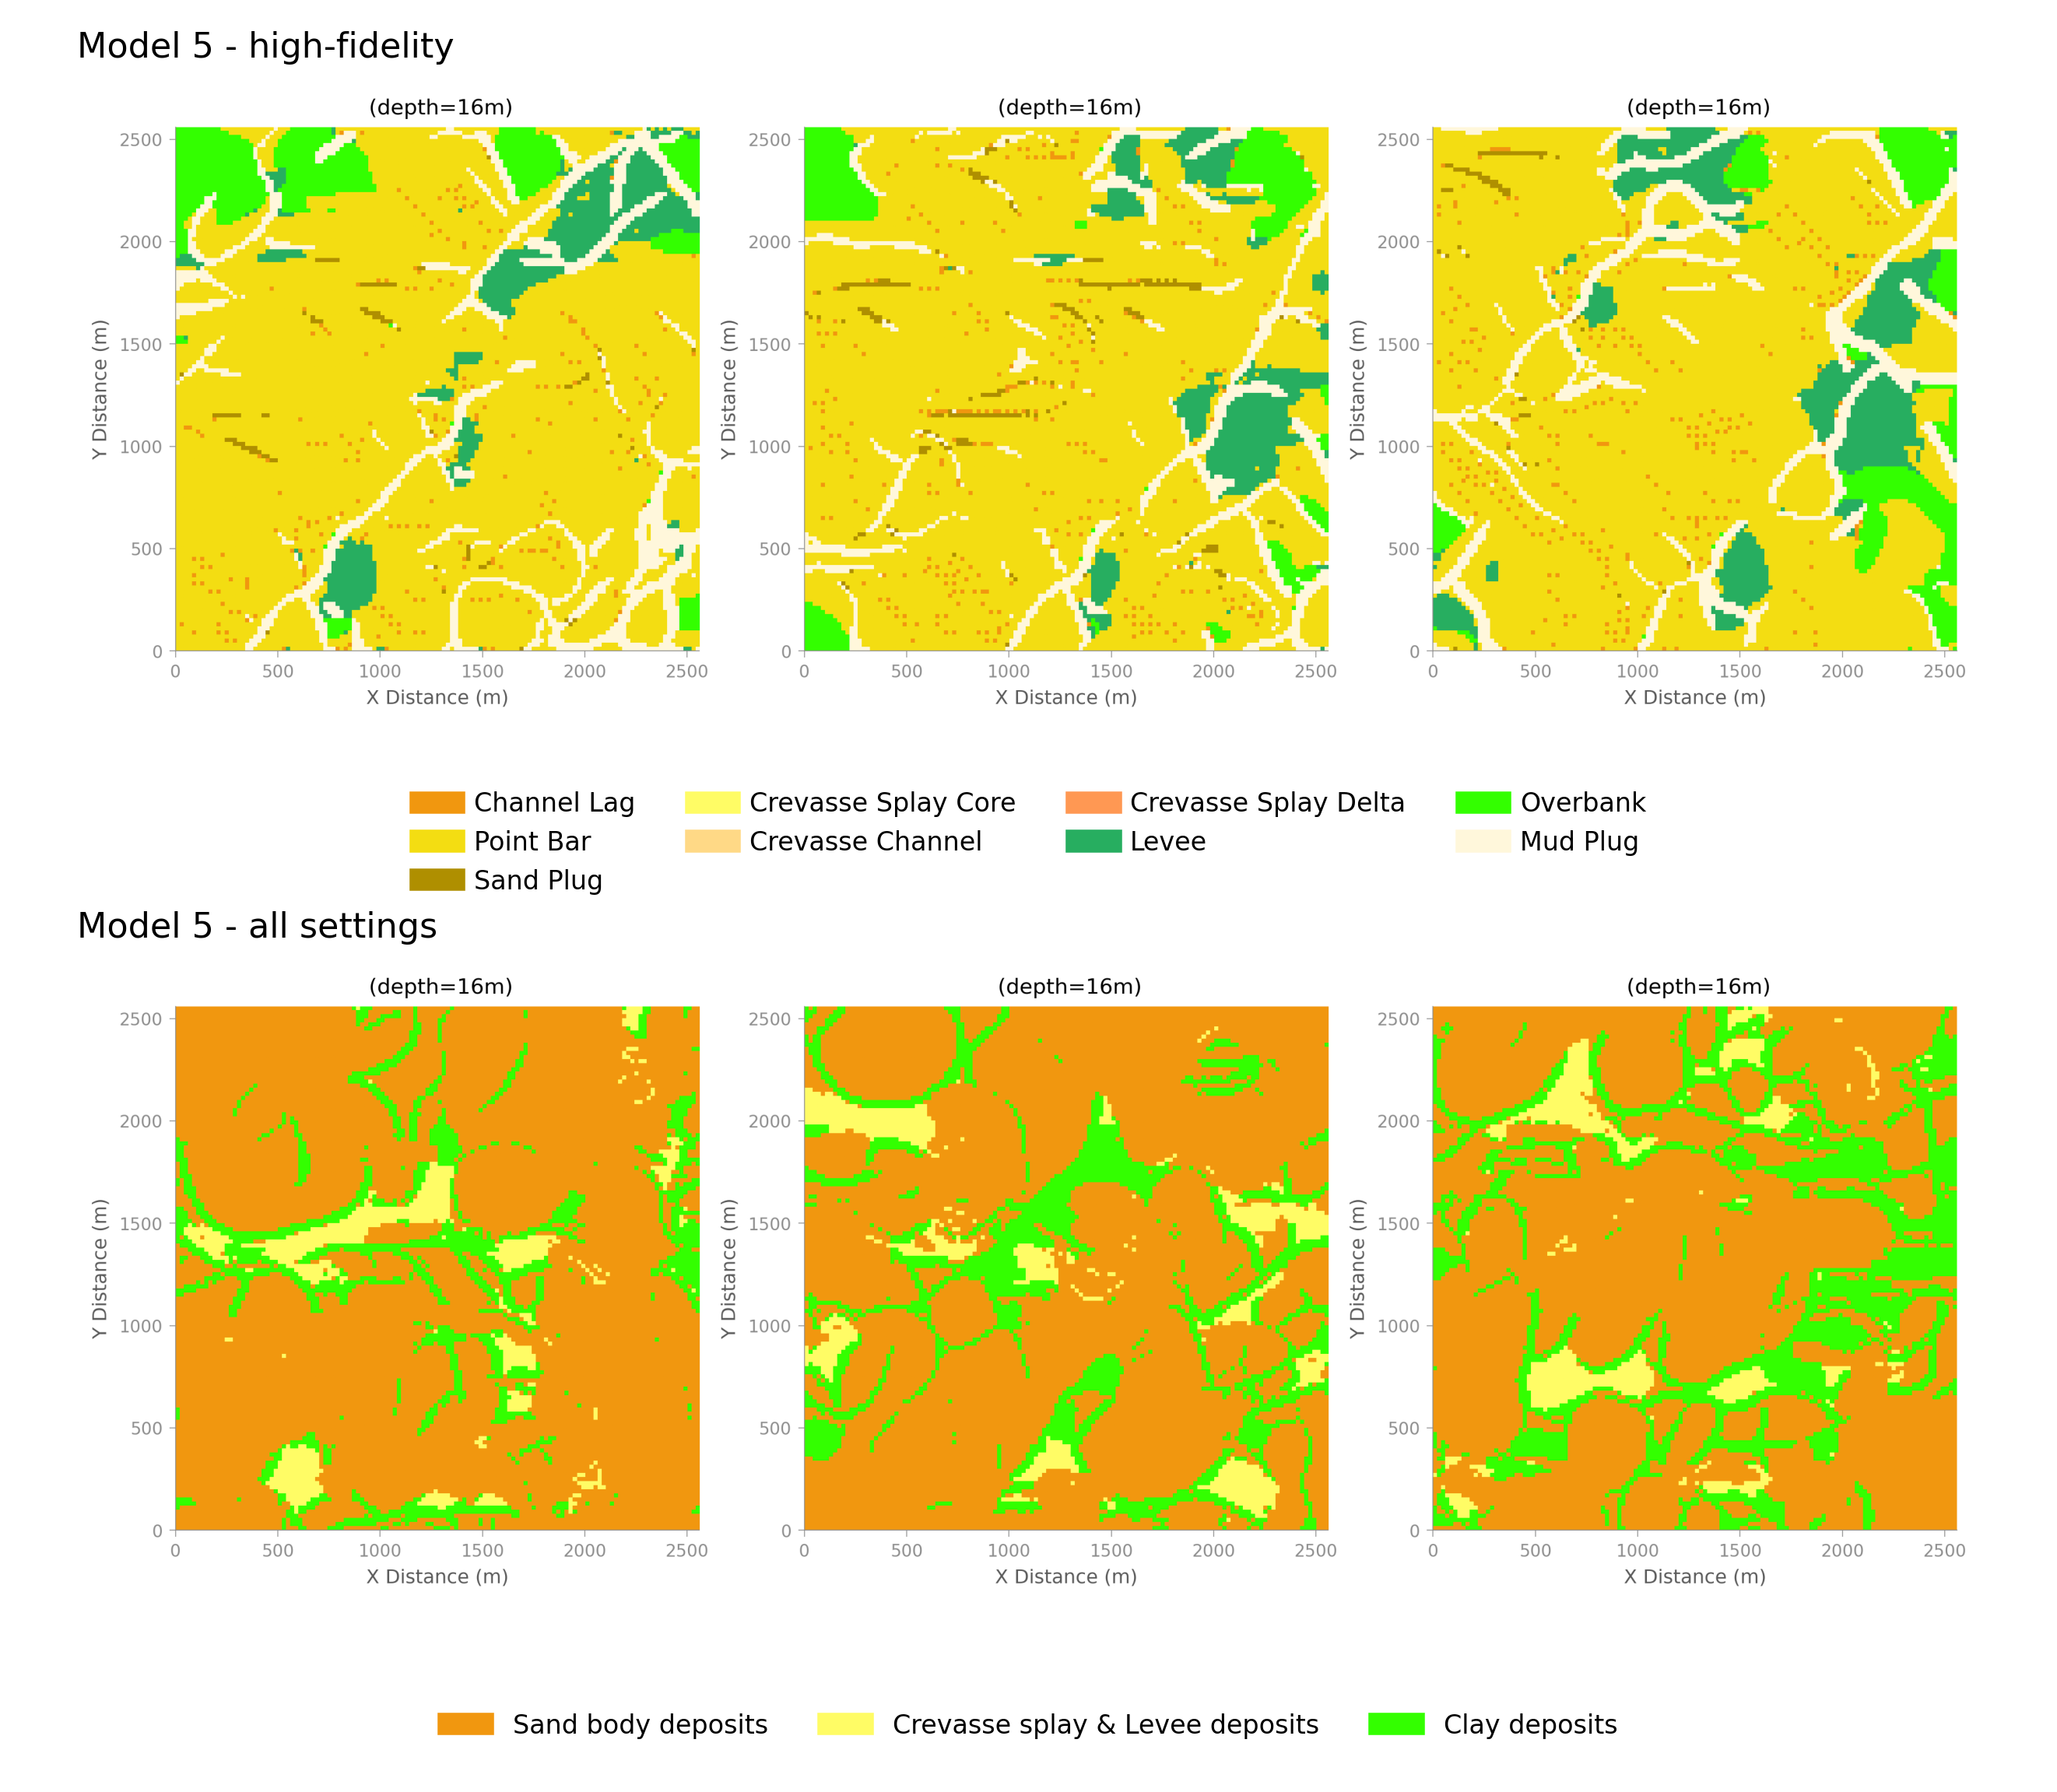
\includegraphics[width=0.99\linewidth]{figures/results/cgan_unconstrained_performance/model_comparison_stacked_legends.png}
    \caption{2D slices taken from the Z-axis at depth 16~m comparing the high-fidelity model (9~classes, Setting~2) and the multi-prior model (3~classes, combined settings).}
    \label{fig:2D_Z_slices_models_hf_all_set_and_flumy}
\end{figure}

\begin{table}[htbp!]
    \centering
    \renewcommand{\arraystretch}{1.4}
    \small
    \begin{tabularx}{\textwidth}{Xccccc}
        \hline
        \textbf{Model Configuration} & \textbf{Epochs} & \textbf{\gls{jsd} $\downarrow$} & \textbf{\gls{msswd} $\downarrow$} & \textbf{Mean $H_{norm} \uparrow$} & \textbf{$n$ Unique Patterns} \\
        \hline
        Setting 2 (grouped)     & -  & -      & -       & 0.692 & 2,949,220 \\
        Setting 2 (non-grouped) & -  & -      & -       & 0.695 & 8,864,195 \\
        High-Fidelity (9-Class, Setting 2)  & 25 & 0.1102 & -       & 0.351 & 6,017,855 \\
        Multi-Prior (Grouped, All Settings) & 25 & \textbf{0.0168} & - & \textbf{0.661} & 4,512,631 \\
        \hline
    \end{tabularx}
    \caption{Overview of evaluation metrics comparing the high-fidelity and multi-prior configurations against the baseline implementations ($N = 100$~realizations).}
    \label{tab:high_fidelity_multiprior_comparison}
\end{table}

Retaining all nine individual facies classes results in substantial mode collapse due to extreme class imbalance. Although the high-fidelity model generates all nine facies volumetrically~(Figure~\ref{fig:app_facies_dist_high_fidelity_model}), it produces numerous isolated channel lag voxels and poorly connected mud and sand plug geometries (Figure~\ref{fig:2D_Z_slices_models_hf_all_set_and_flumy}). Mean normalized spatial entropy collapses to 0.351 (compared to 0.695 in the non-grouped baseline), accompanied by a 32\%~drop in unique patterns ($6.01\text{M}$ vs.~$8.86\text{M}$, Table~\ref{tab:high_fidelity_multiprior_comparison}) and an elevated \gls{jsd} of 0.1102. Equal-weight loss functions encourage the generator to focus predominantly on the dominant point bar facies while failing to properly structure rare minority classes.

Training on an unconditioned multi-prior dataset destabilizes GAN convergence and causes structural mode collapse. The generator outputs repetitive, quasi-identical realizations that fail to capture the distinct architectural features of Settings~1, 2, or 3 (Figure~\ref{fig:2D_Z_slices_models_hf_all_set_and_flumy}). Although the global \gls{jsd} appears low (0.0168) due to dataset-wide statistical averaging, spatial entropy is suppressed ($\bar{H}_{norm} = 0.661$) and visual diversity is largely lost. Mixing conflicting fluvial rules without explicit conditional input labels creates ambiguous gradients for the discriminator, collapsing the latent representation into a single averaged pattern.

\begin{figure}[htbp]
    \centering
    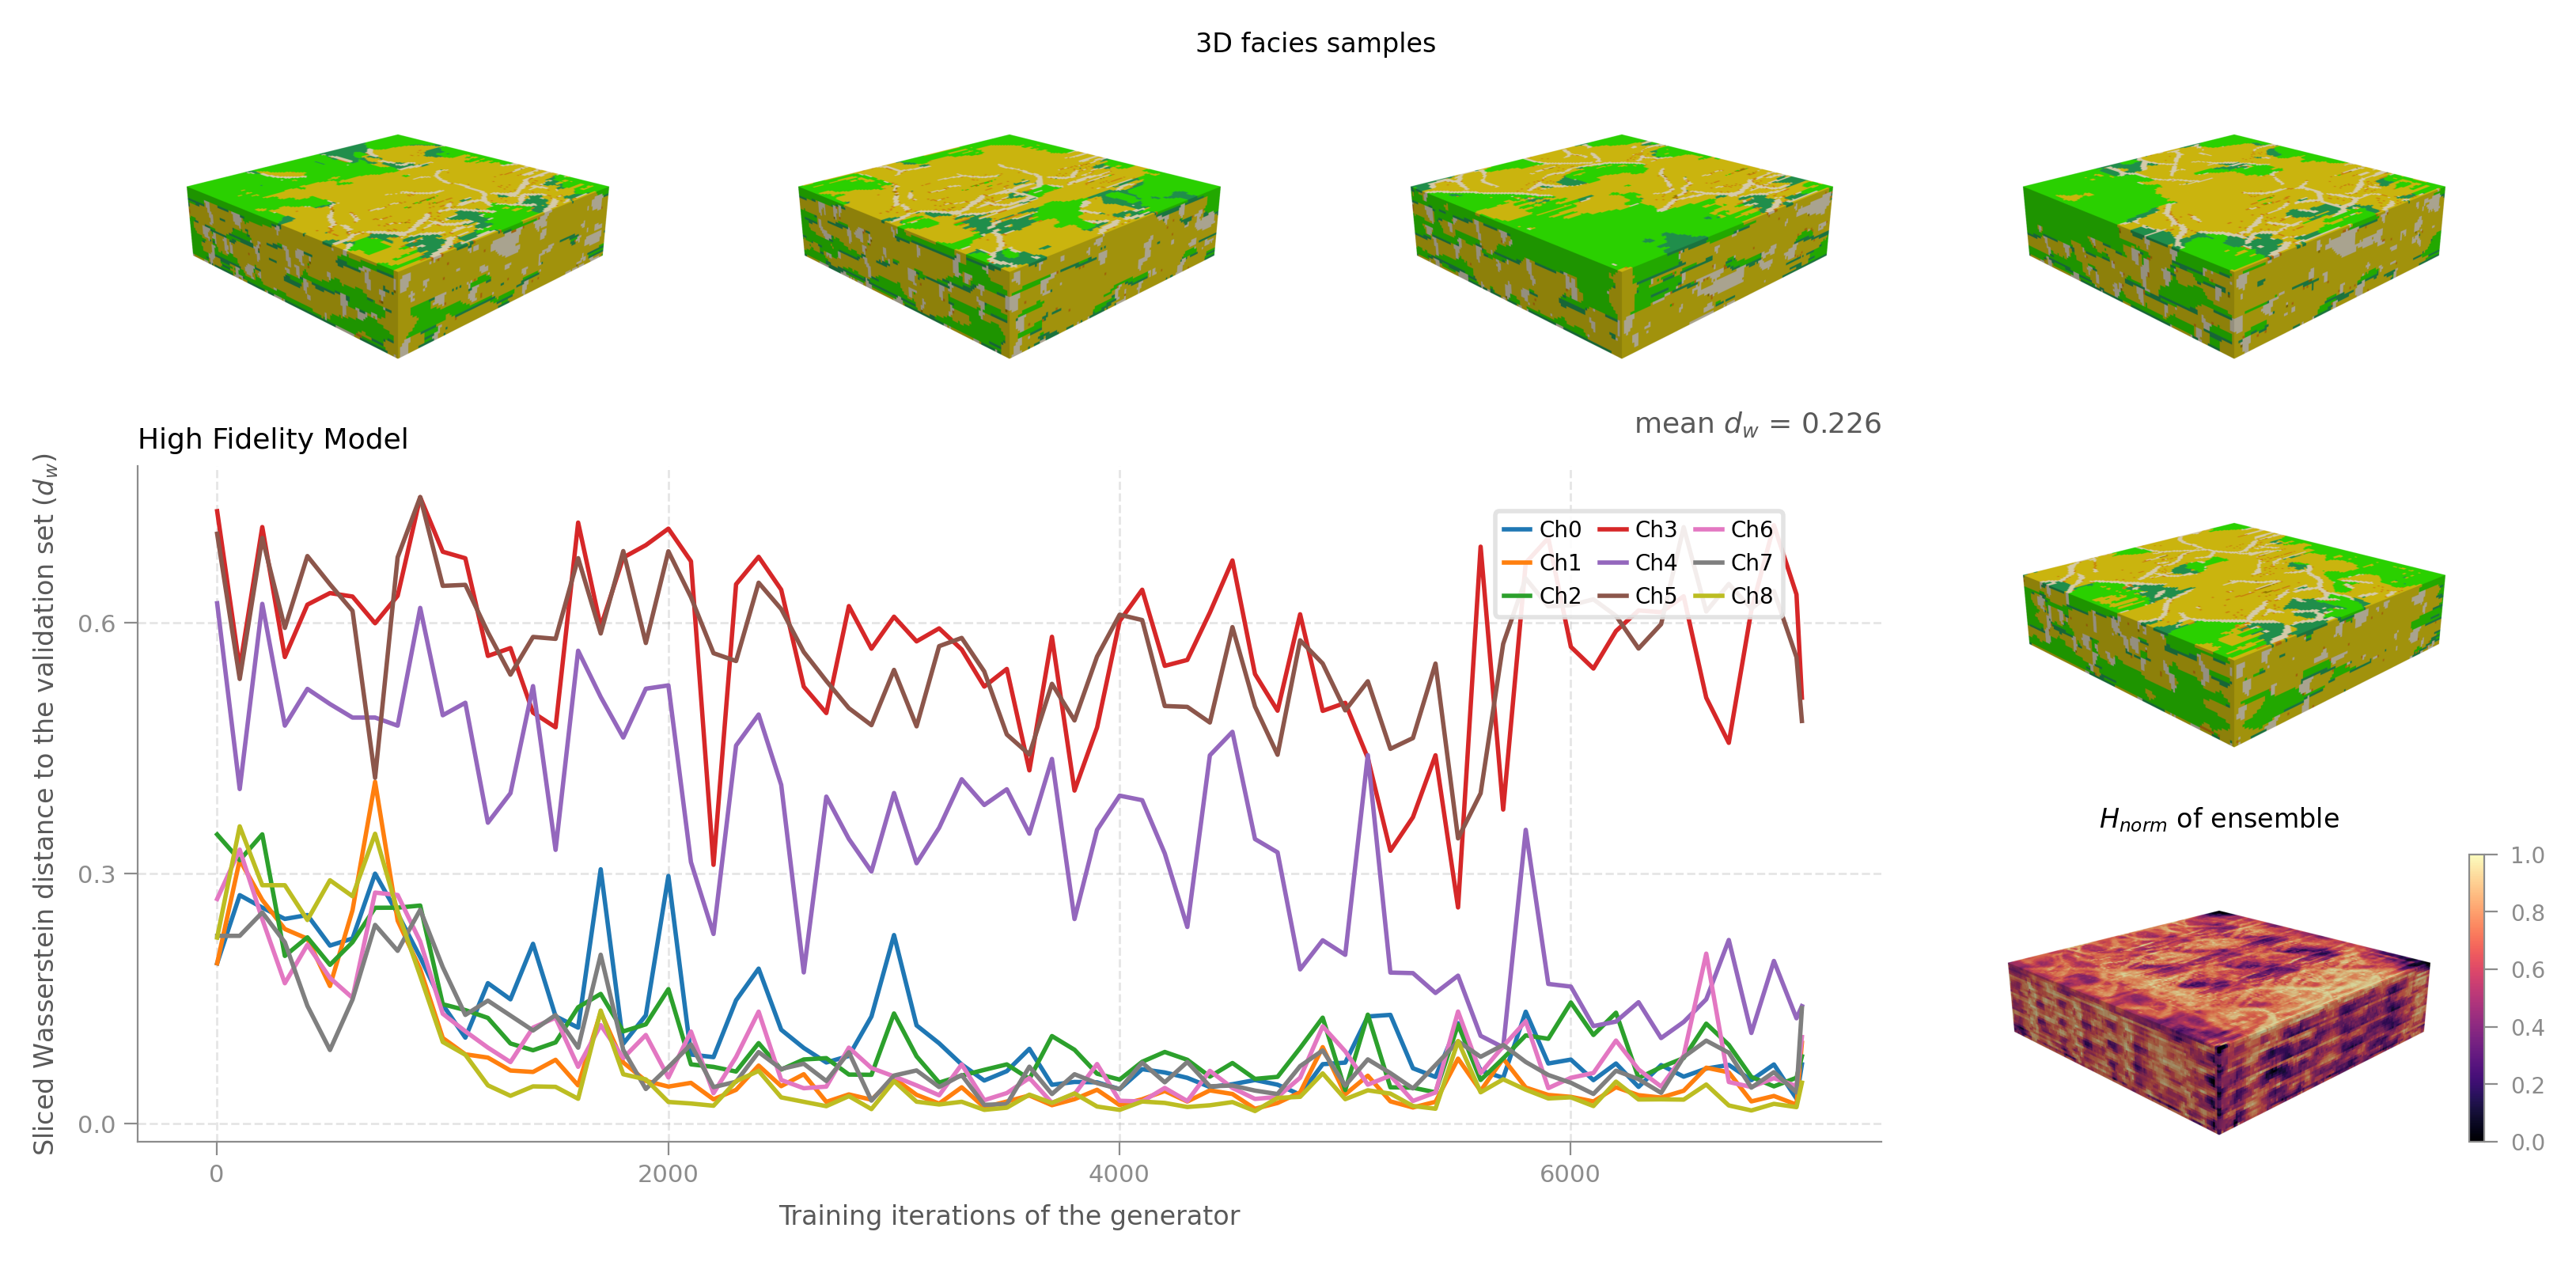
\includegraphics[width=0.90\textwidth]{figures/results/cgan_unconstrained_performance/combined_plot_all_channels.png}
    \caption{Overview of the high-fidelity model metrics and training evolution over 25~epochs.}
    \label{fig:combined_plot_all_channels}
\end{figure}

Channel-by-channel \gls{swd} loss curves explain the underlying failure modes across individual facies in the 9-class model. Abundant facies, including Point Bar (Channel~1), Overbank (Channel~7), and Mud Plug (Channel~8), converge rapidly to low \gls{swd} values ($<0.05$, Figure~\ref{fig:combined_plot_all_channels}). In contrast, heavily suppressed minority facies, such as Crevasse Splay Core (Channel~3) and Crevasse Splay Delta (Channel~5), show flat \gls{swd} curves ($>0.60$) with virtually no learning progress across 25~epochs. Channel~4 (Crevasse Channel) displays a steady downward trend, suggesting that intermediate facies might benefit from targeted class-weighting or extended training.

Directly applying the Model~5 hyperparameter setup to 9-class or multi-prior datasets is insufficient for stable multi-modal learning. The Model~5 configuration was optimized specifically for the 3-class, single-setting problem and did not undergo dedicated ablation for more complex data distributions. Higher categorical dimensions and multi-modal priors alter the training dynamics, leading to class suppression and mode collapse. Future applications involving multi-prior or high-fidelity datasets will require dedicated hyperparameter tuning, class-weighted loss formulations, or conditional GAN architectures.

\section{Post-Inversion Results}\label{Sec:Post_Cond_Res}
A fully trained Model~5 generator was inverted using well data from DEL-GT-01 and DEL-GT-02-S2 to evaluate conditioned realization quality. The first 32~metres of both wells capture contrasting depositional environments: DEL-GT-01 lacks Overbank Mudstone, whereas DEL-GT-02-S2 contains almost no Levee deposits (Figure~\ref{fig:well_data}). This asymmetry tests the framework's ability to adapt to distinct localized constraints rather than defaulting to an average regional pattern. For each configuration, 100~latent vectors were optimized via \gls{lso} (requiring $\sim 1.5$~hours) and subsequent \gls{pv} (requiring an additional $\sim 2.5$~hours) to generate conditioned subsurface realizations (loss curves detailed in Figure~\ref{fig:appendix_post_lso_losses}).

\subsection{Latent Space Optimization}
Conditioning accuracy during Latent Space Optimization responds positively to the spatial constraint threshold ($Th$). Increasing the threshold radius from $Th=1$ to $Th=5$ increases the mean Macro F1-score from 0.70 to 0.84 (Table~\ref{tab:optimization_f1_scores}). This improvement occurs across all three facies classes, with the dominant sand ($C1$) increasing from 0.77 to 0.90, and the minority class ($C2$) rising from 0.56 to 0.79. Expanding the spatial radius of the context loss mask provides gradient descent with sufficient spatial leverage to locate latent vectors that better honor hard well constraints.

\begin{table}[htbp!]
    \centering
    \renewcommand{\arraystretch}{1.4}
    \small
    \begin{tabularx}{\textwidth}{X c c c c c c c}
        \hline
        \textbf{Model} & \textbf{Th} & $\mathbf{\overline{\vphantom{\big|}\text{Macro F1}}\uparrow}$ & $\mathbf{\overline{\vphantom{\big|}F1}_{C1}\uparrow}$ & $\mathbf{\overline{\vphantom{\big|}F1}_{C2}\uparrow}$ & $\mathbf{\overline{\vphantom{\big|}F1}_{C3}\uparrow}$ & \textbf{\gls{jsd}}$\downarrow$ & $\mathbf{\overline{\vphantom{\big|}H}_{norm}\uparrow}$ \\
        \hline
        Run 1 (\gls{lso}) & 1 & 0.70 & 0.77 & 0.56 & 0.76 & 0.015 & 0.686  \\
        Run 2 (\gls{lso}) & 2 & 0.78 & 0.84 & 0.68 & 0.81 & 0.017 & 0.685  \\
        Run 3 (\gls{lso}) & 5 & 0.84 & 0.90 & 0.79 & 0.85 & 0.028 & 0.663  \\
        \hline
    \end{tabularx}
    \caption{Latent Space Optimization (LSO) performance metrics across varying spatial constraint thresholds ($Th$) evaluated on DEL-GT-01 and DEL-GT-02-S2 ($N = 100$~realisations).}
    \label{tab:optimization_f1_scores}
\end{table}

\gls{lso} conditioning performance depends significantly on latent vector initialization, leading to wide performance distributions. While Model~3 ($Th=5$) achieves the highest proportion of realizations with $\text{F1} > 0.8$, individual realization scores span a wide range from 0.50 to 0.95 across all threshold settings (Figure~\ref{fig:post_optimization_f1_scores_distributions}). This variability corresponds directly to the optimization loss curves (Figure~\ref{fig:appendix_post_lso_losses}), where final loss values vary by up to an order of magnitude depending on the starting latent seed. Because gradient descent is susceptible to local minima in complex latent spaces, multi-start optimizations are necessary to consistently identify high-fidelity conditioned realizations.

\begin{figure}[htbp!]
    \centering
    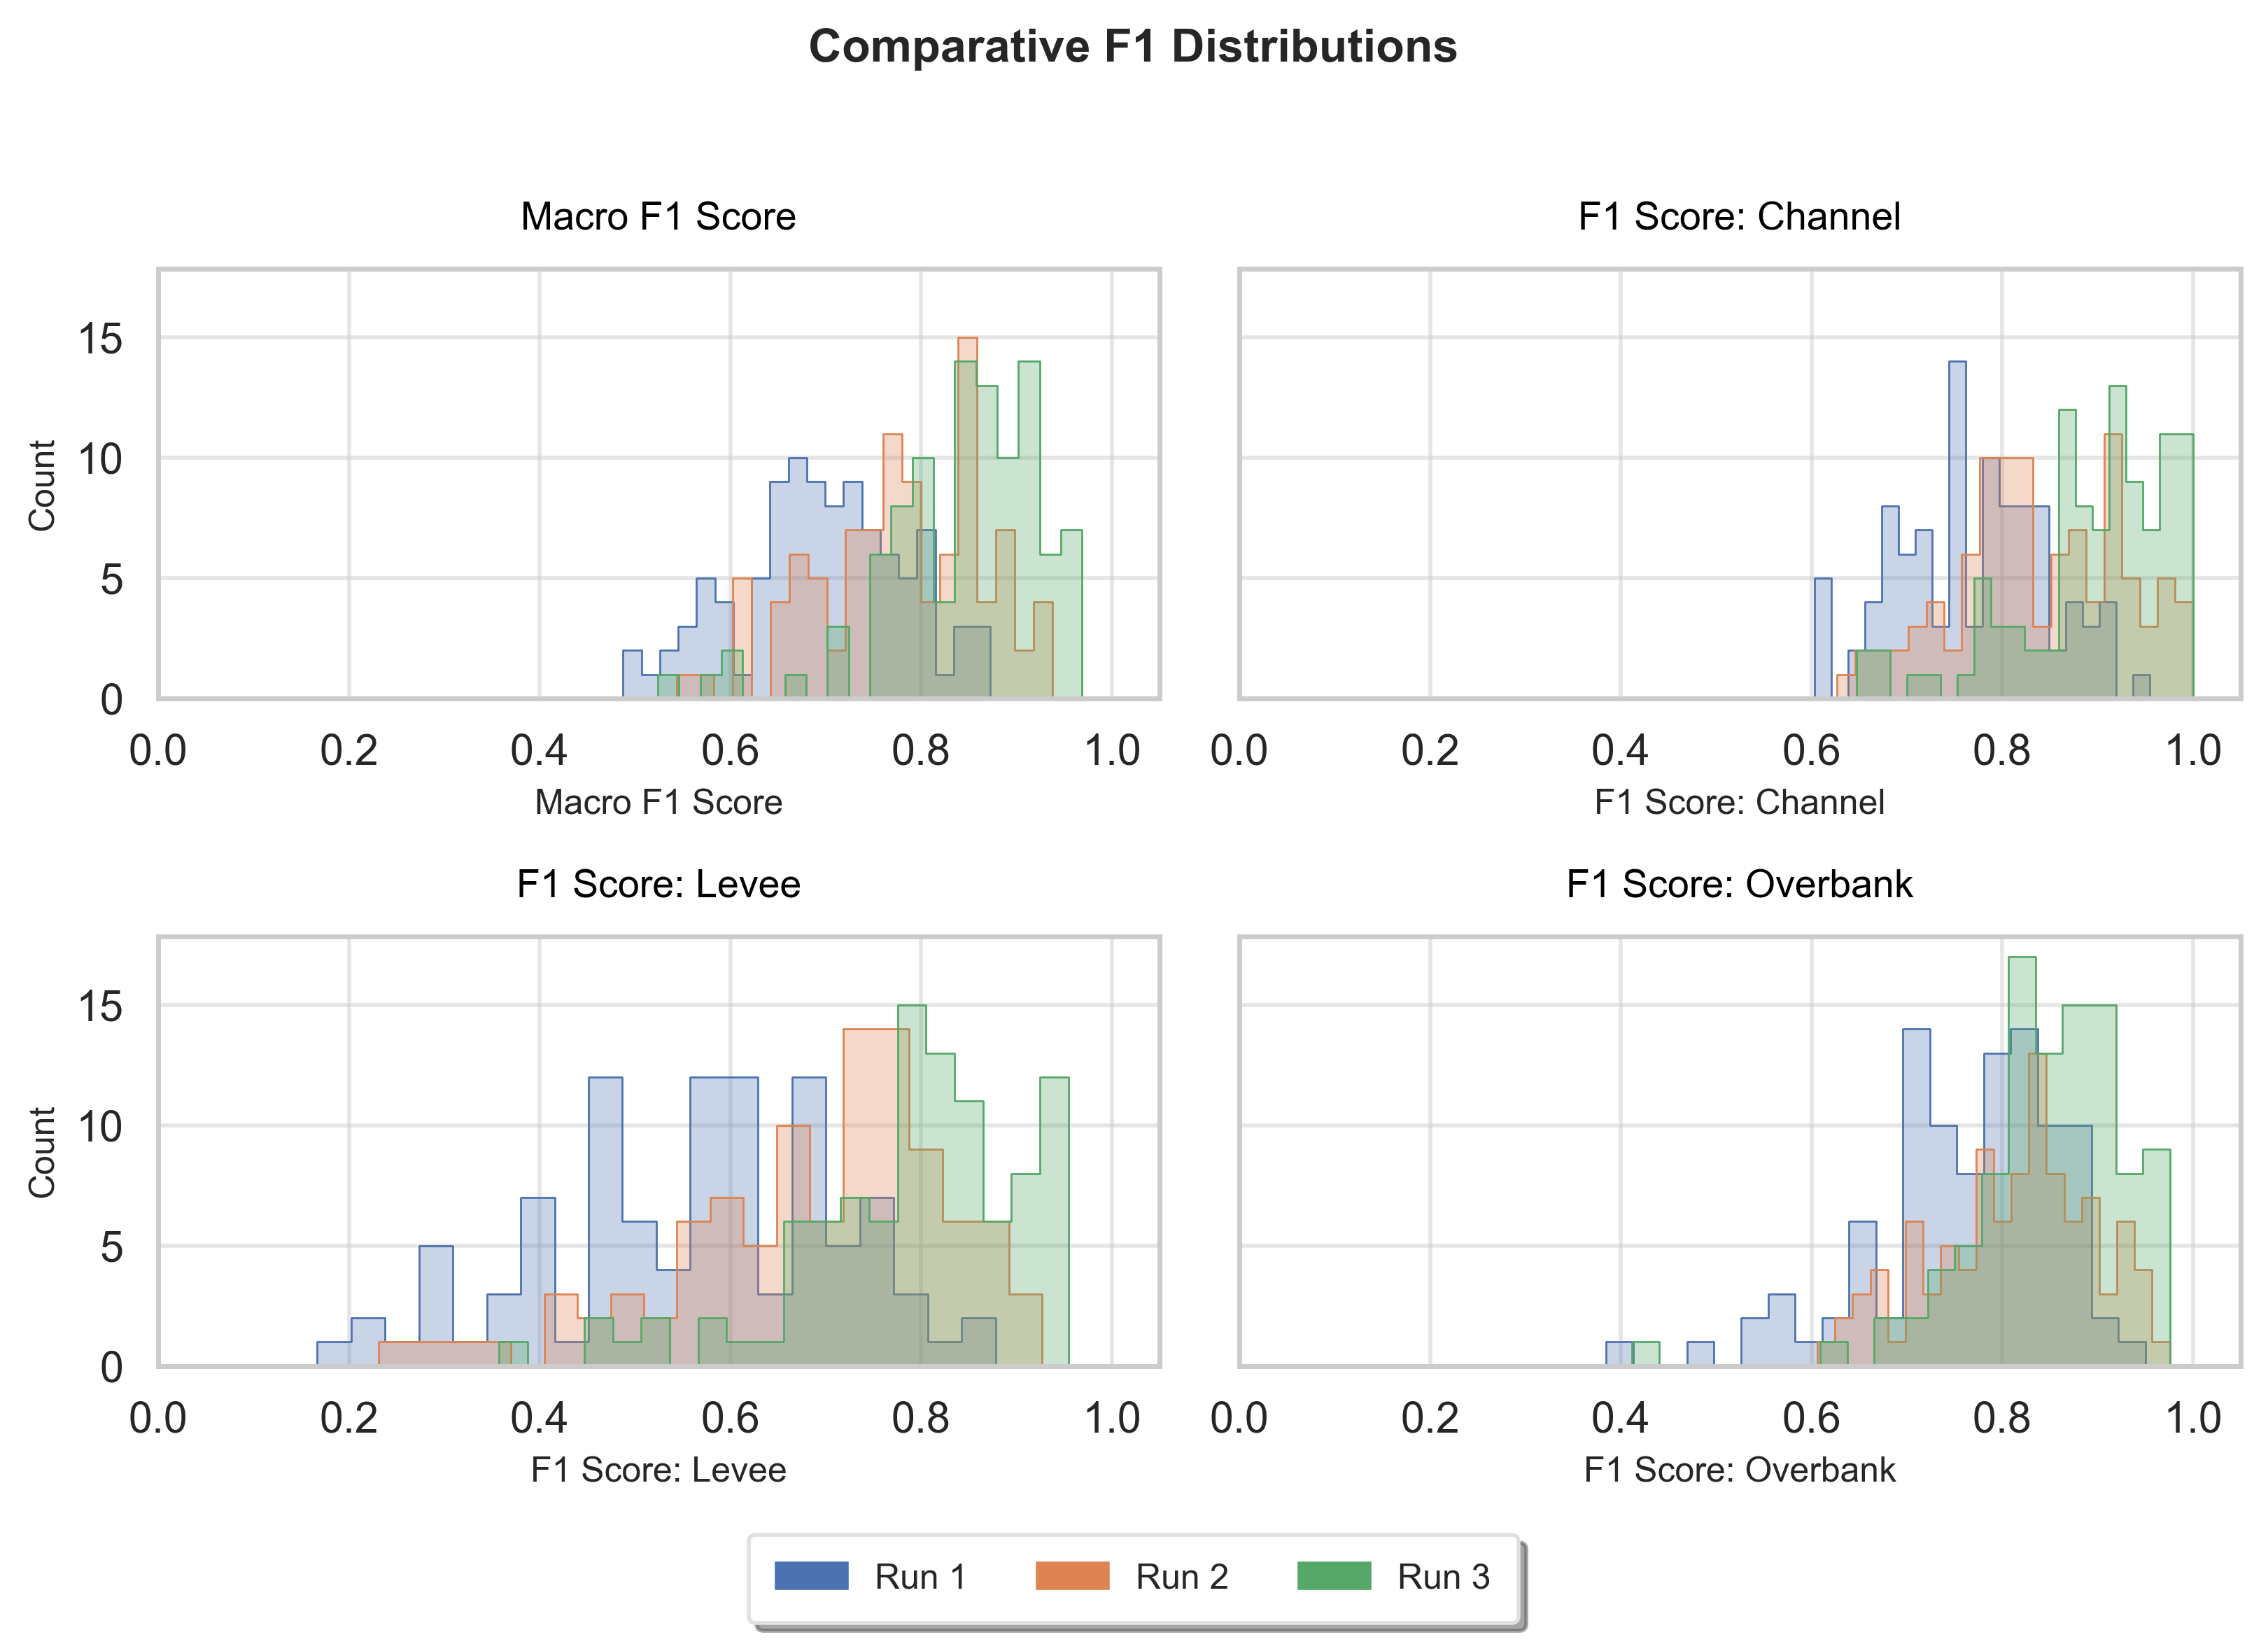
\includegraphics[width=0.9\textwidth]{figures/results/cgan_constrained_performance/f1_score_comparisons.png}
    \caption{Macro F1 and single channel F1 score distributions for three optimization models with varying threshold values (Model~1: threshold = 1, Model~2: threshold = 2, and Model~3: threshold = 5).}
    \label{fig:post_optimization_f1_scores_distributions}
\end{figure}

Vertical depth profiles demonstrate that conditioning accuracy is closely linked to the prior volumetric proportions of the training facies. In thick intervals of dominant channel sand (FA1)—such as the 15~m basal sand package in DEL-GT-01 ($-17$~m to $-32$~m)—ensemble probabilities stay pinned near $1.0$, resulting in near-complete match accuracy (Figure~\ref{fig:post_optimization_metrics_across_Z_axis}). Conversely, thin interbedded layers of minority crevasse and levee deposits (FA2) in DEL-GT-02-S2 represent a noticeable optimization bottleneck, with prediction probabilities peaking at only $\sim 0.7$ and dropping to $0.3$ in logged sections. Clay deposits (FA3) show intermediate, consistent replication, confirming that the generator's conditioning reliability reflects the class representation established during prior training.

\begin{figure}[htbp!]
    \centering
    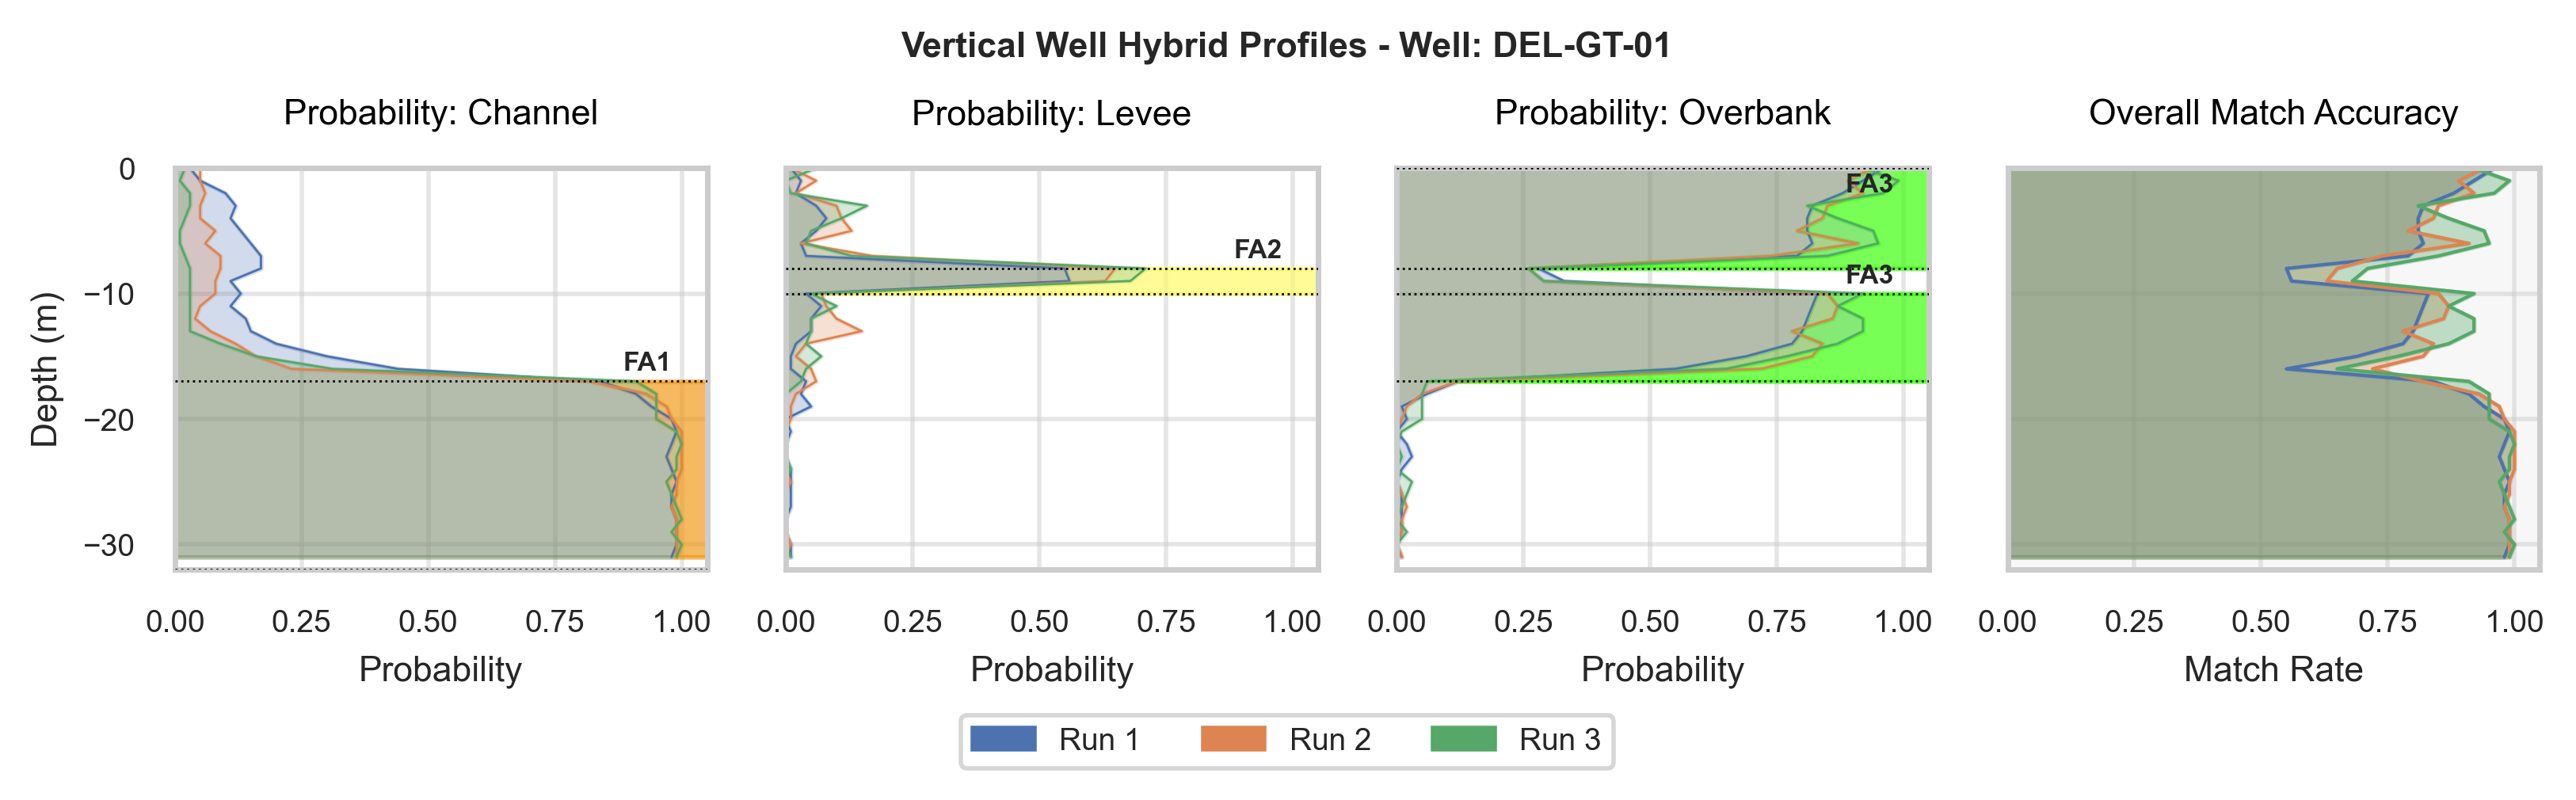
\includegraphics[width=0.95\textwidth]{figures/results/cgan_constrained_performance/accuracy_score_across_depth_DEL-GT-01.png}
    \vspace{0.3cm}
    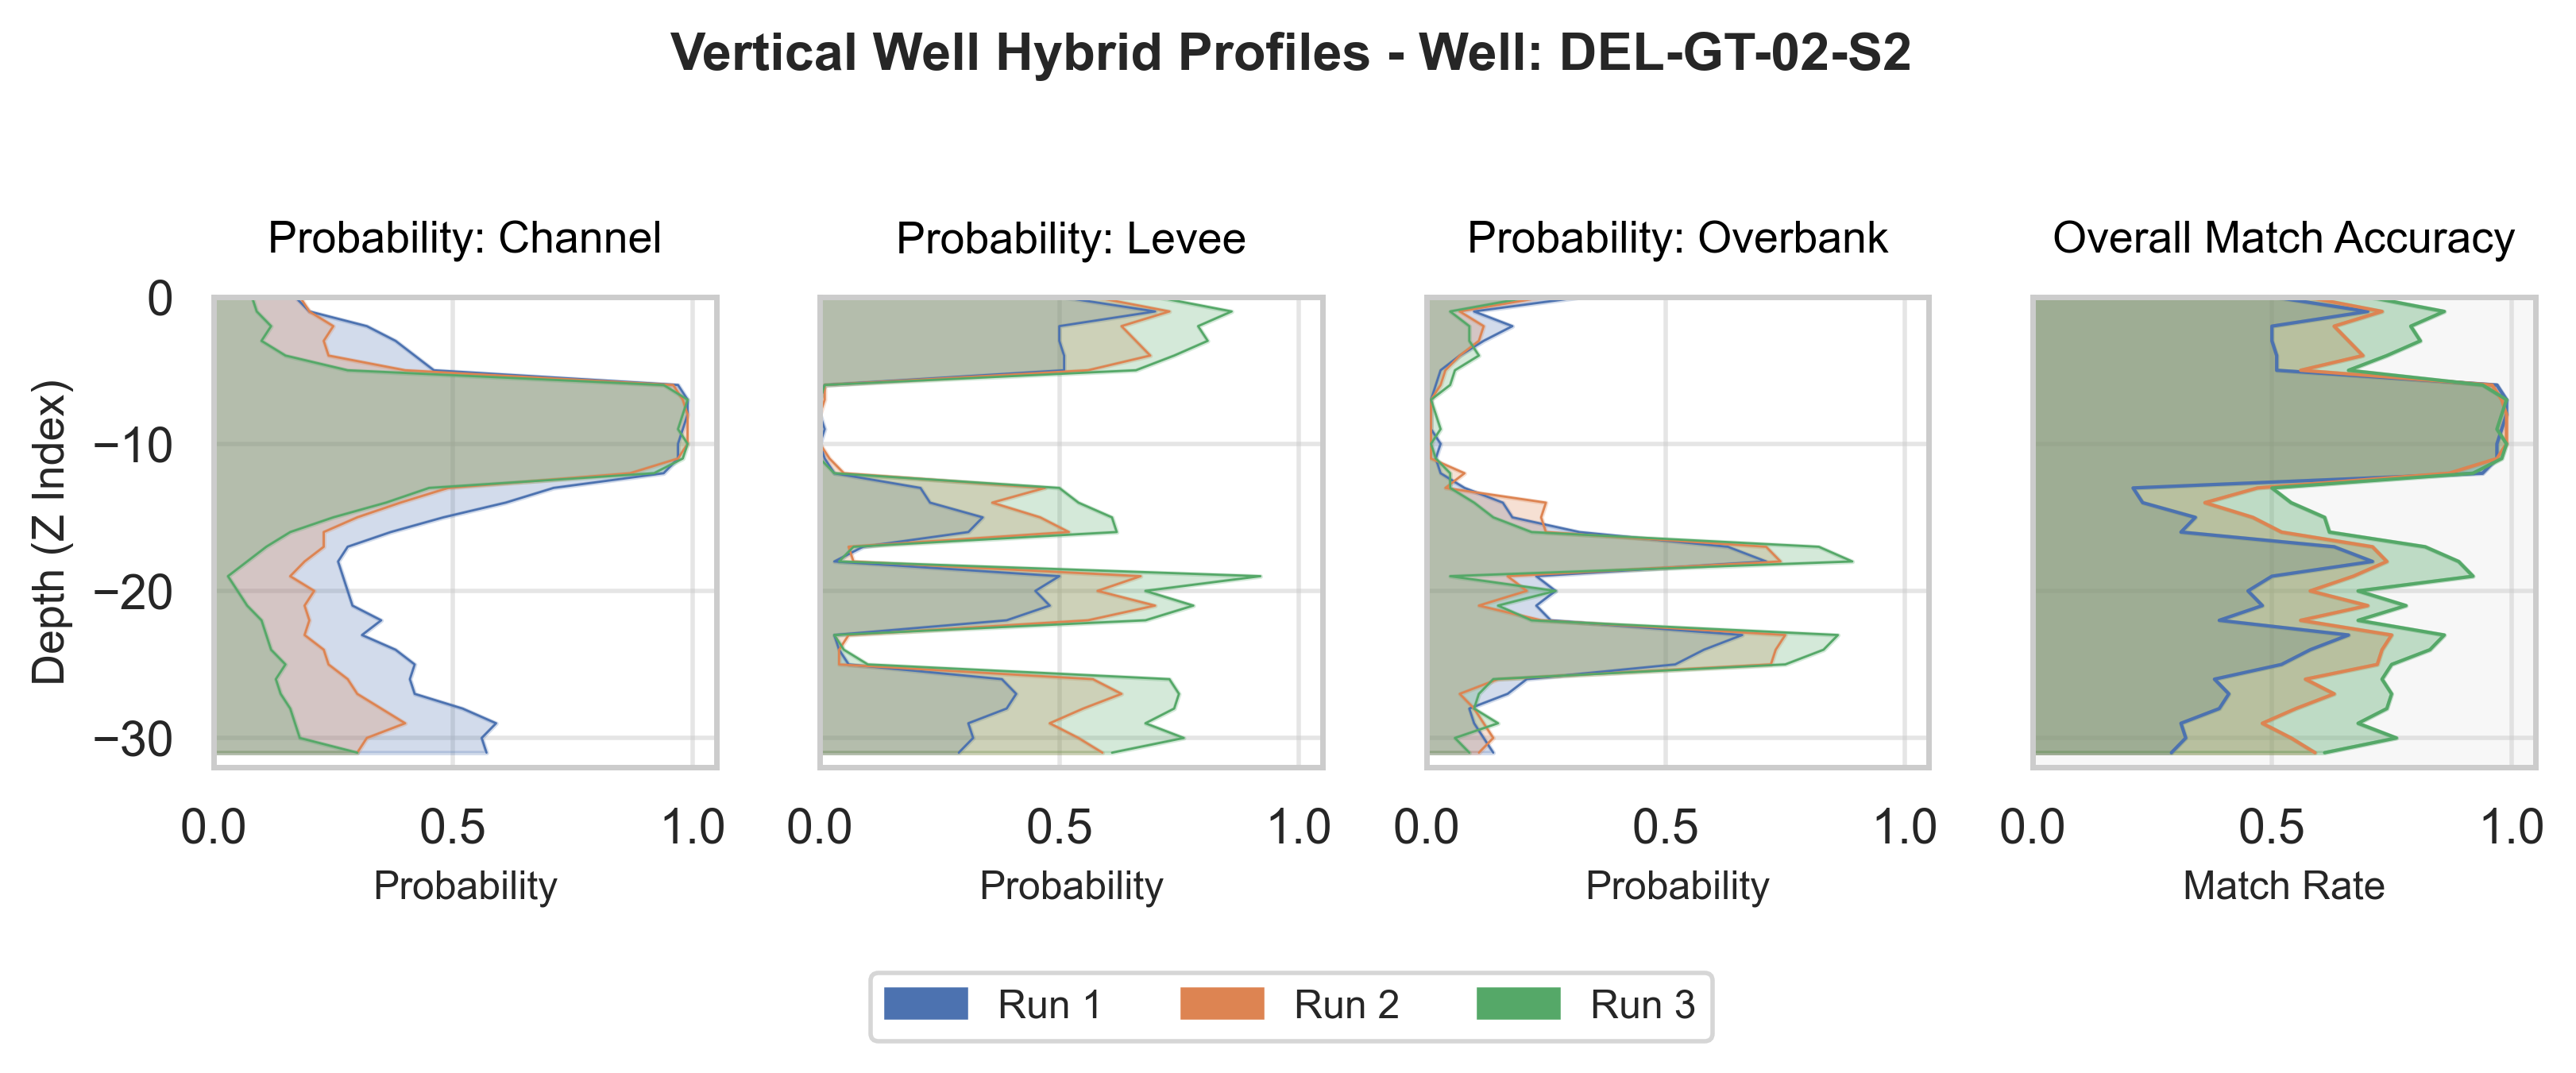
\includegraphics[width=0.95\textwidth]{figures/results/cgan_constrained_performance/accuracy_score_across_depth_DEL-GT-02-S2.png}
    \caption{Vertical depth profiles for Wells DEL-GT-01 (top row) and DEL-GT-02-S2 (bottom row). The left three panels display ensemble prediction probabilities for each facies alongside black dotted lines indicating the exact interval along the well that the facies is found. Shaded color intervals highlight the distance between the prediction curve and perfect probability ($1.0$), directly illustrating how strongly each model respects the well constraints at that depth. The rightmost panel shows the aggregated match accuracy across the three evaluated optimization runs.}
    \label{fig:post_optimization_metrics_across_Z_axis}
\end{figure}

Widening the \gls{lso} constraint threshold introduces an inherent trade-off between conditioning accuracy and ensemble spatial entropy. As the mean Macro F1-score increases from 0.70 to 0.84, normalized spatial entropy ($\bar{H}_{norm}$) decreases from 0.686 ($Th=1$) to 0.663 ($Th=5$, Table~\ref{tab:optimization_f1_scores}). Applying a larger spatial constraint forces an expanding radial volume around each wellbore to remain deterministic across the realization ensemble (Figure~\ref{fig:2D_XY_slices_at_well_trajectories}). In horizontal cross-sections ($XY$), this low-entropy halo expands isotropically, whereas in vertical sections ($XZ/YZ$), it assumes an elliptical geometry due to vertical grid scaling.

\begin{figure}[htbp!]
    \centering
    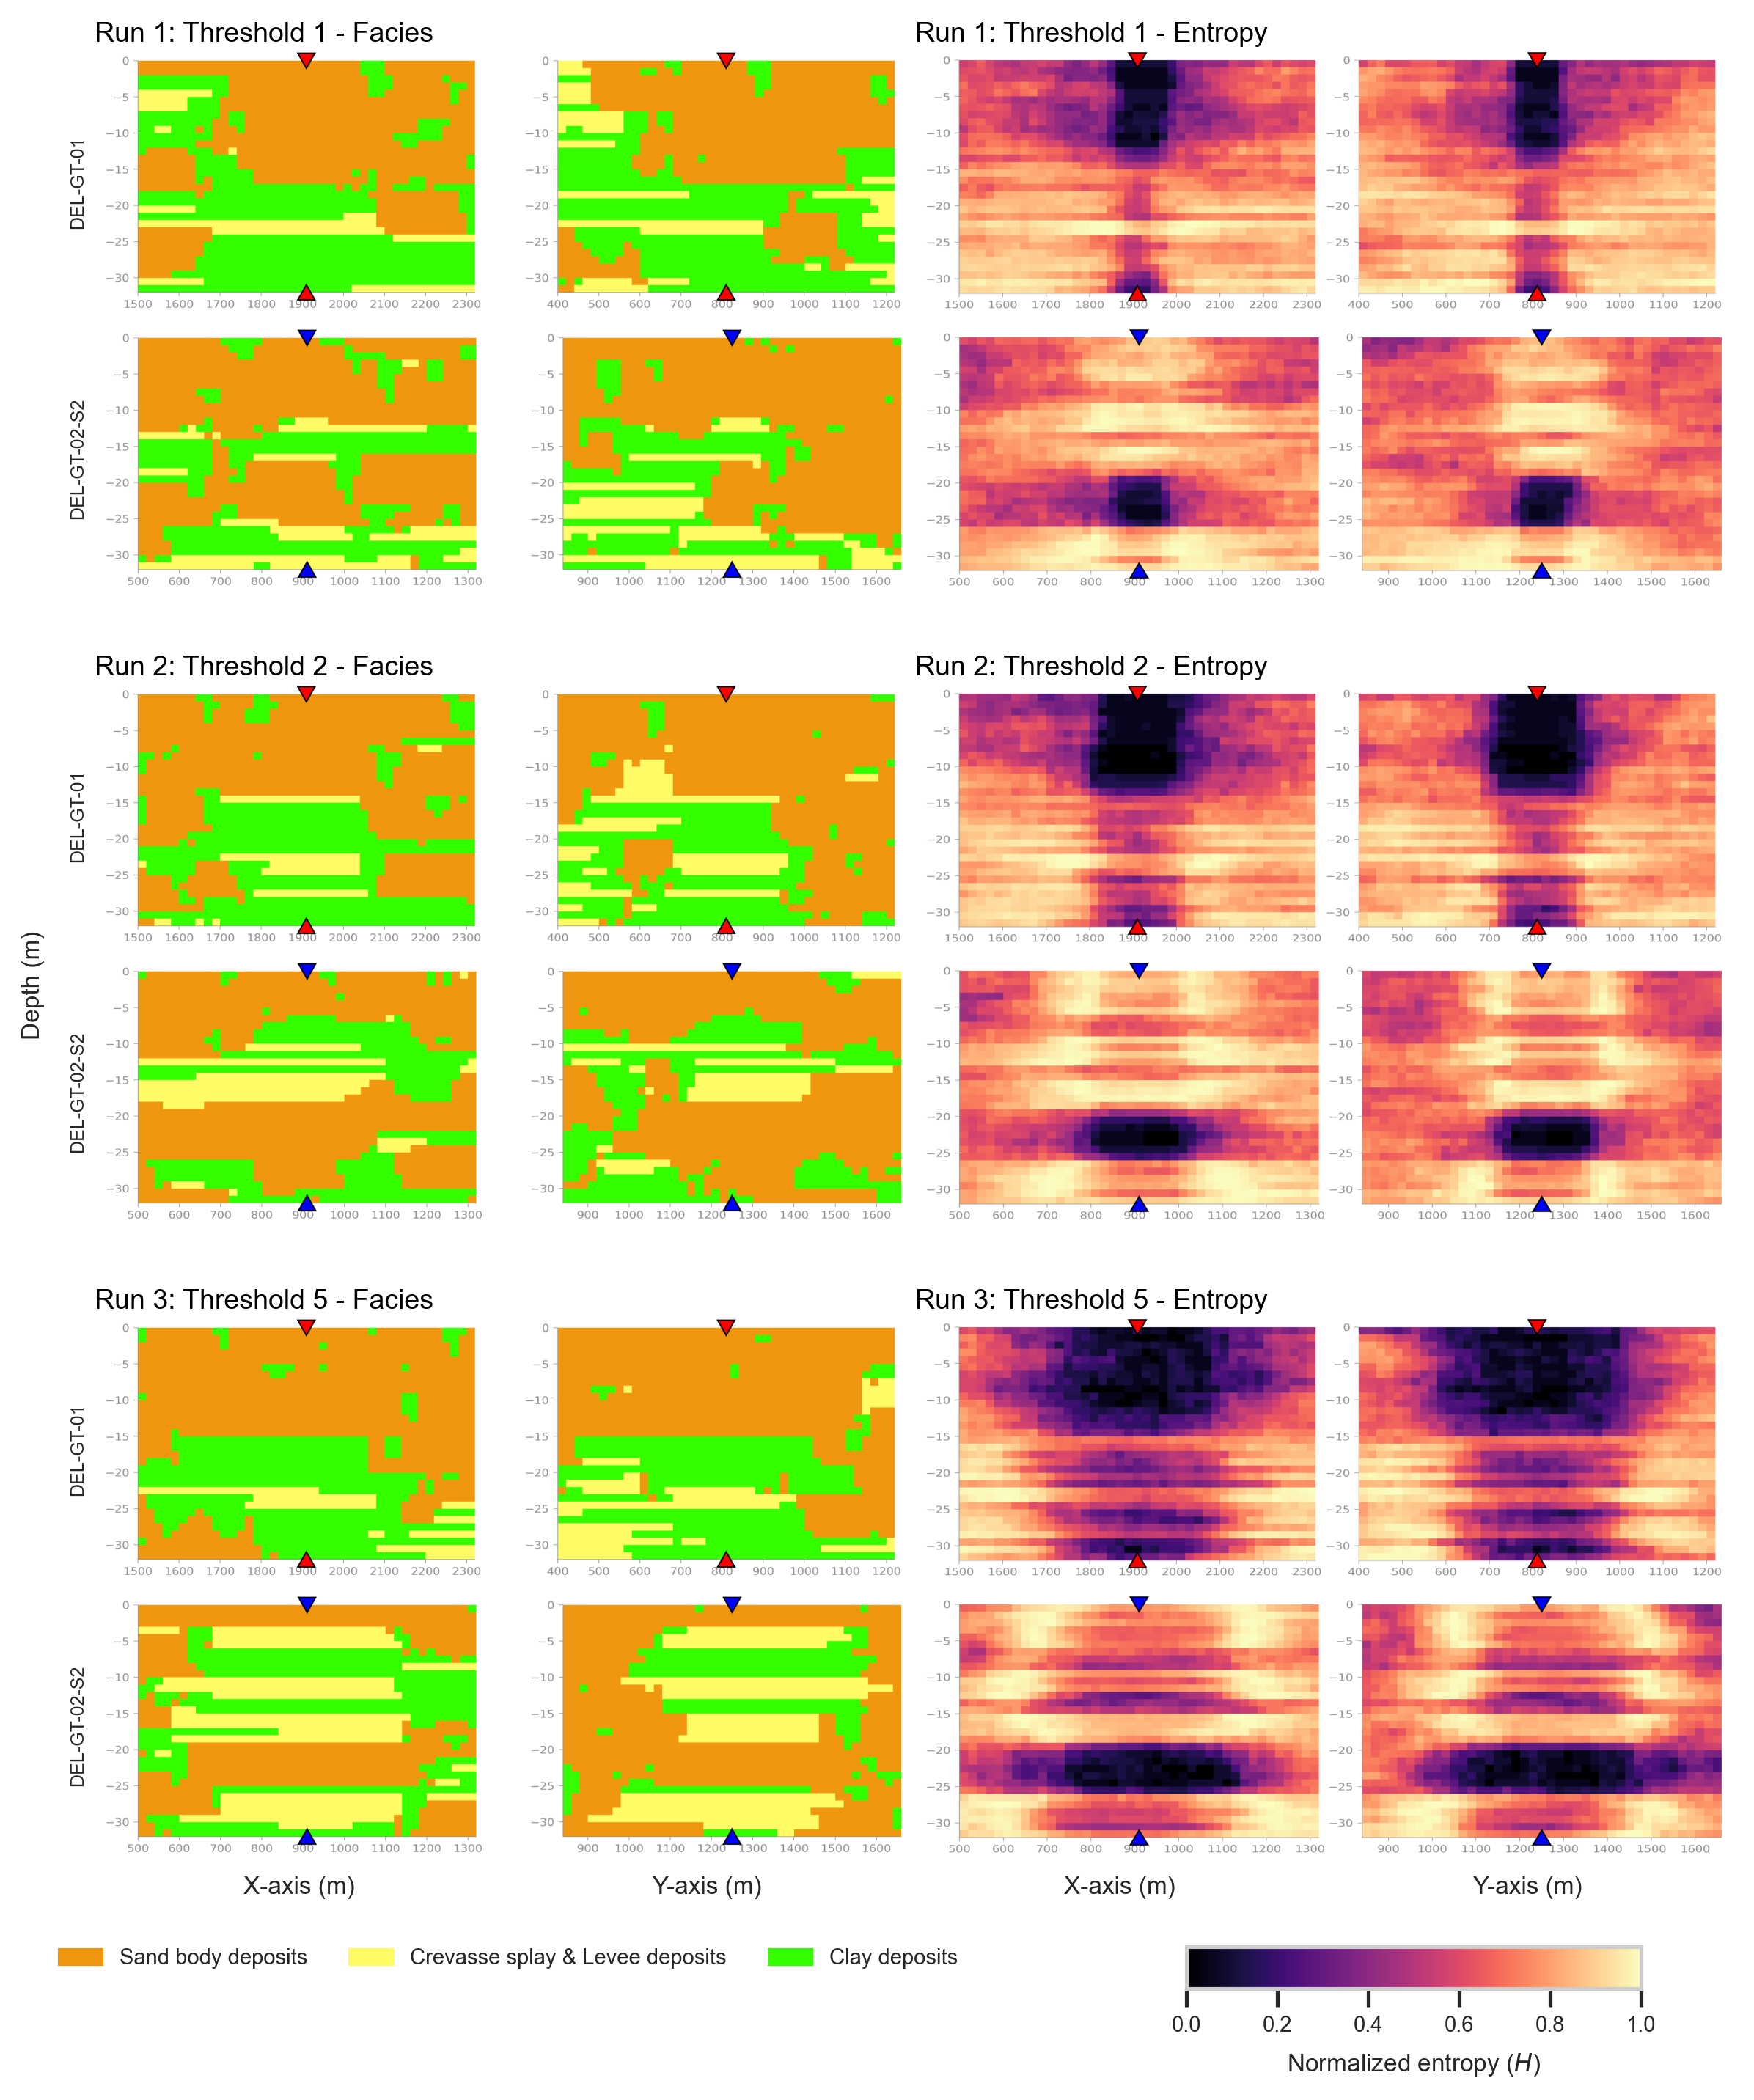
\includegraphics[width=1.05\linewidth]{figures/results/cgan_constrained_performance/master_grouped_facies_and_entropy_post_lso.png}
    \caption{Post-\gls{lso} 2D slices of the facies and voxel-wise entropy taken of the realisations. Well trajectories are indicated by the red~\triangled[red] (producer) and blue~\triangled[blue] (injector) triangles. The threshold, a hyperparameter of the~\gls{lso}, increases with each run (Run~1: th = 1, Run~2: th = 2, Run~3: th = 5) which has a strong correlation to the regions with decreased voxel-wise entropy. The figure has a $\pm$~20$\times$ exaggeration of the Z-axis.}
    \label{fig:2D_XY_slices_at_well_trajectories}
\end{figure}

Forcing large \gls{lso} thresholds ($Th=5$) can induce localized stratification and alter nearby geological structures. In the upper section of DEL-GT-02-S2, wide thresholds cause over-expanded FA2 and FA3 constraint zones to suppress the continuous FA1 sand body (Figure~\ref{fig:2D_XY_slices_at_well_trajectories}). This localized distortion increases global distribution divergence, raising \gls{jsd} from 0.015 ($Th=1$) to 0.028 ($Th=5$). These observations indicate that \gls{lso} alone cannot achieve perfect conditioning without compromising local geological realism, motivating the use of Pivotal Tuning.

\pagebreak
\subsection{Pivotal Tuning}
Pivotal Tuning addresses the minority-class conditioning bottleneck without requiring wide spatial constraint thresholds. Applying \gls{pv} to the tightly constrained baseline ($Th=1$) raises the mean Macro F1-score from 0.70 to 0.89 (Table~\ref{tab:pivotal_tuning_f1_scores}). The minority class ($C2$) F1-score increases from 0.56 to 0.87, outperforming even the widest \gls{lso} configuration ($Th=5$). Furthermore, increasing the \gls{pv} threshold to $Th=5$ yields only marginal gains (Macro F1 reaches 0.91), indicating that once generator weights are fine-tuned, a compact context window is sufficient for effective conditioning.

\begin{table}[htbp!]
    \centering
    \renewcommand{\arraystretch}{1.4}
    \small
    \begin{tabularx}{\textwidth}{X c c c c c c c}
        \hline
        \textbf{Model} & \textbf{Th} & $\mathbf{\overline{\vphantom{\big|}\text{Macro F1}}\uparrow}$ & $\mathbf{\overline{\vphantom{\big|}F1}_{C1}\uparrow}$ & $\mathbf{\overline{\vphantom{\big|}F1}_{C2}\uparrow}$ & $\mathbf{\overline{\vphantom{\big|}F1}_{C3}\uparrow}$ & \textbf{\gls{jsd}}$\downarrow$ & $\mathbf{\overline{\vphantom{\big|}H}_{norm}\uparrow}$ \\
        \hline
        Run 1 (\gls{pv})  & 1 & 0.89 & 0.90 & 0.87 & 0.89 & 0.017 & 0.714 \\
        Run 2 (\gls{pv})  & 2 & 0.90 & 0.92 & 0.89 & 0.89 & 0.018 & 0.702 \\
        Run 3 (\gls{pv})  & 5 & 0.91 & 0.96 & 0.90 & 0.91 & 0.029 & 0.671 \\
        \hline
    \end{tabularx}
    \caption{Pivotal Tuning (PV) performance metrics across varying spatial constraint thresholds ($Th$) evaluated on DEL-GT-01 and DEL-GT-02-S2 ($N = 100$~realisations).}
    \label{tab:pivotal_tuning_f1_scores}
\end{table}

Pivotal Tuning eliminates uncertainty along the well trajectories while preserving high spatial entropy across the inter-well reservoir domain. A sharp, single-voxel column of near-zero entropy forms directly along the trajectories of DEL-GT-01 and DEL-GT-02-S2 (Figure~\ref{fig:2D_XY_slices_at_well_trajectories_pv}). Away from the wellbores, the inter-well region maintains a high spatial entropy ($\bar{H}_{norm} = 0.714$ for $Th=1$), exceeding the entropy of all \gls{lso} configurations. For wider thresholds ($Th=2$ and $Th=5$), the low-entropy zone spreads into the surrounding reservoir, reducing global entropy to 0.671 in Run~3.

\begin{figure}[htbp!]
    \centering
    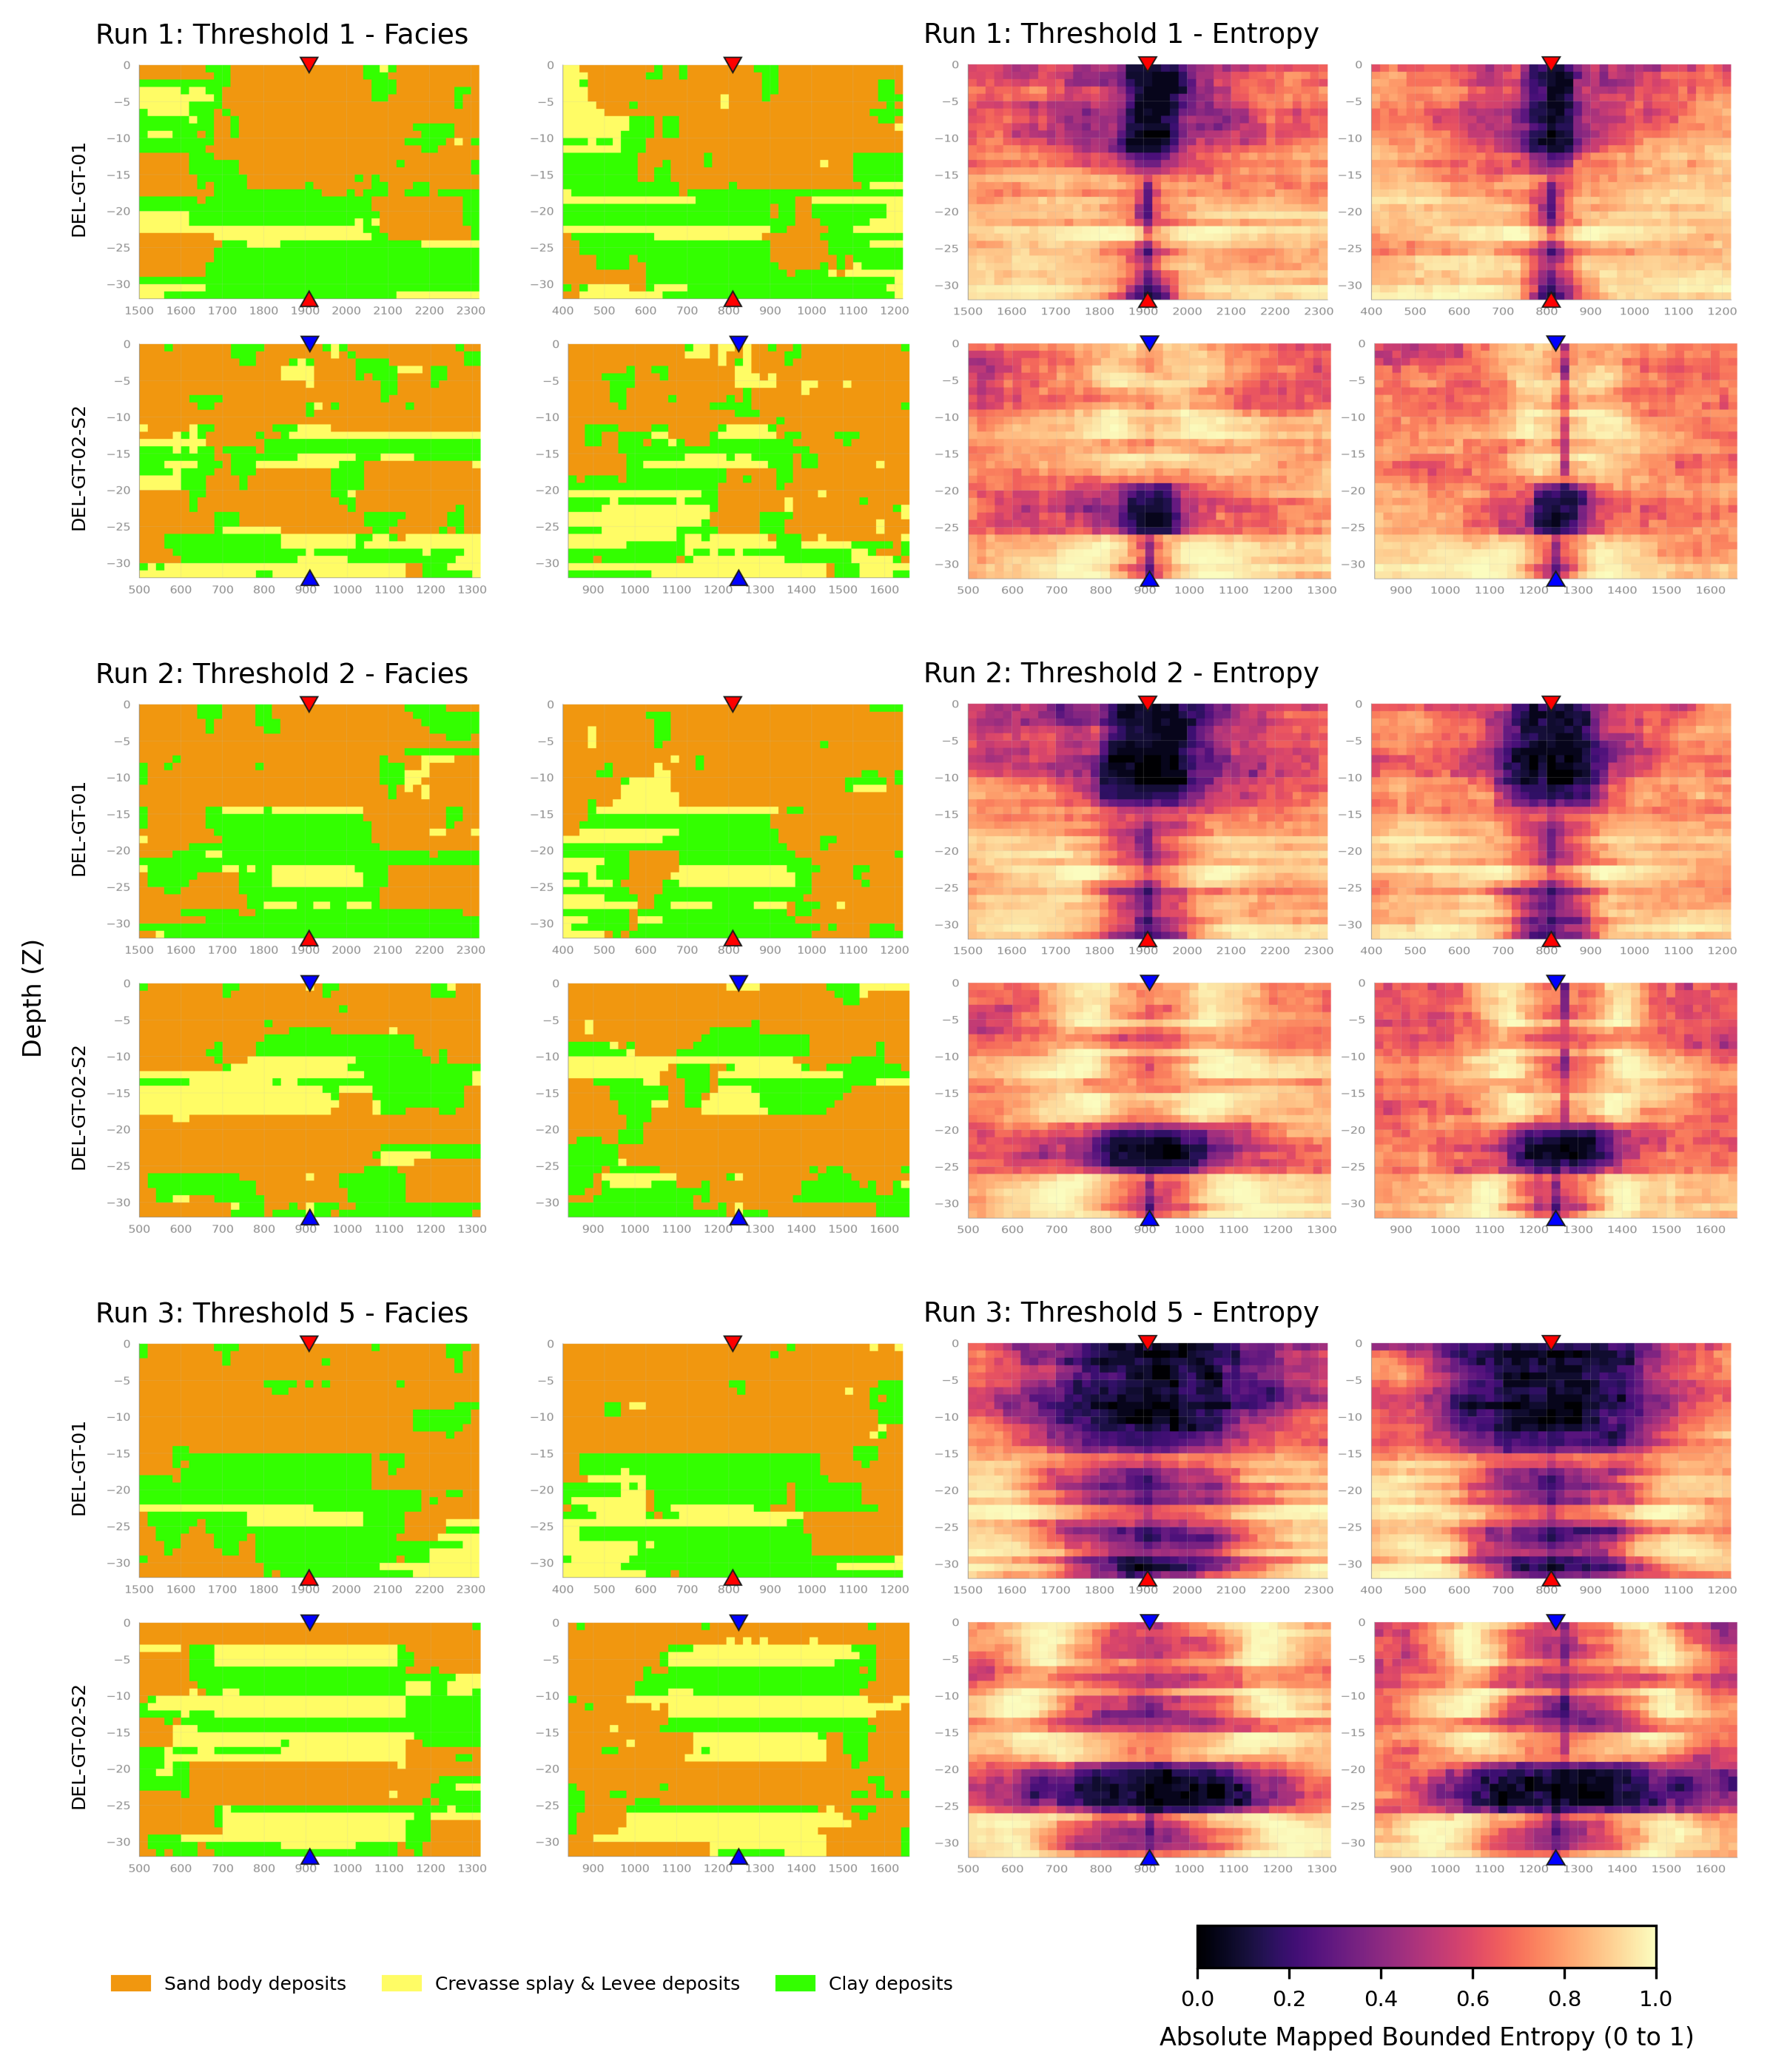
\includegraphics[width=1.05\linewidth]{figures/results/cgan_constrained_performance/master_grouped_facies_and_entropy_post_pv.png}
    \caption{Post-\gls{pv} 2D slices of the facies and voxel-wise entropy taken of the realisations. Well trajectories are indicated by the red~\triangled[red] (producer) and blue~\triangled[blue] (injector) triangles. The threshold, a hyperparameter of the optimization, increases with each run (Run~1: th = 1, Run~2: th = 2, Run~3: th = 5) which correlates with the regions of decreased voxel-wise entropy. The figure has a $\pm$~20$\times$ exaggeration of the Z-axis.}
    \label{fig:2D_XY_slices_at_well_trajectories_pv}
\end{figure}

While Pivotal Tuning achieves near-deterministic well matching, fine-tuning at wider thresholds introduces localized morphological artifacts. 2D facies cross-sections at $Th=5$ display blocky facies boundaries, isolated single voxels, and localized distortions near the well trajectories (Figure~\ref{fig:2D_XY_slices_at_well_trajectories_pv}). These localized modifications coincide with an increase in global distribution divergence, with \gls{jsd} rising to 0.029 at $Th=5$. Consequently, the $Th=1$ configuration offers the most suitable operational balance, providing strong well accuracy (0.89 F1), high inter-well spatial entropy (0.714), and minimal structural distortion.
